%Vorlage von Klaus Prüger kprueger{at}uni-bremen.de, 2021
\documentclass[	pdfLatex, 
								a4paper,
								12pt, DIV11, BCOR5mm,
								parskip,
								%openany,
								] {scrreprt}
\usepackage[utf8]{inputenc}


\usepackage{hyperref}
\usepackage{comment}
\usepackage[ngerman]{babel}
\usepackage[nonumberlist,toc,acronym]{glossaries}
\usepackage{fancyhdr}
\usepackage[section]{placeins}
\usepackage{graphicx}
\usepackage{listings}
\usepackage{bibgerm}
\usepackage{varwidth}
\usepackage{float}
\usepackage{natbib}

\usepackage{epstopdf}
\usepackage{textpos}
\usepackage{changepage}
\usepackage{theorem}
\usepackage{caption}
\usepackage{framed}
\usepackage{booktabs}
\usepackage{tikz}
\usetikzlibrary{decorations.markings,arrows,positioning,trees,calc,fit,shapes}
\usepackage[noend]{algorithmic}
\usepackage{algorithm}
\usepackage{environ}
\usepackage{xcolor}
\usepackage{url}
\usepackage{todonotes}
\usepackage{listings}




%Kopfzeile hinzufuegen
\renewcommand{\sectionmark}[1]{\markboth{#1}{}} % set the \leftmark

\fancypagestyle{unsrtnat}{
    
    \fancyhead[R]{\leftmark}
    \fancyhead[L]{Job Jimmy Lebelwa Danmou}
    \renewcommand{\headrulewidth}{1pt}
    %\fancyfoot[R]{\thepage}
}

\pagestyle{fancy}

%Literaturverzeichnis hinzufuegen
\bibliographystyle{plain}
%\normalfont
%\scshape

% Glossar hinzufuegen
\makeglossaries

\newglossaryentry{vr}
{
    name=VR,
    description={Virtuelle Realität kurz VR beschreibt das eintauchen und interagieren mit Hilfe einer Brille und Kontrollern in einer computergenerierten Welt}
}

\newglossaryentry{false positive}
{
    name=False Positive,
    description={Ein \textit{False Positive} Befund liegt vor, wenn ein Partikel entdeckt wird, das nicht hätte entdeckt werden dürfen. Denn entweder sind sie zu klein, zu dunkel oder sogar zu viele Detektionskreise um das gleiche Partikel}
}

\newglossaryentry{false negative}
{
    name=False Negative,
    description={Ein \textit{False Negative} Befund liegt vor, wenn ein Partikel nicht entdeckt wird, das hätte entdeckt werden müssen.}
}

%%%%%%%%%%%%%%%%%%%%%%%%%%
%Dokument Beginn
%%%%%%%%%%%%%%%%%%%%%%%%%%

\begin{document}
\setcounter{page}{-2}
\pagestyle{empty}
\pagenumbering{none}

%Formalien
%Deckblatt Daten
\newcommand{\firstreviewer}{Reviewer 1}
\newcommand{\secondreviewer}{Reviewer 2}
\newcommand{\supervisor}{Betreuer:in}
\newcommand{\thesistype}{Bachelorarbeit}
\newcommand{\myauthor}{Vorname Nachname}
\newcommand{\mymaintitle}{Platzhalter}
\newcommand{\mysubtitle}{Untertitel Platzhalter} 
\newcommand{\mytitle}{\centering {\Huge \mymaintitle}\\[.3in] 
    {\Large \mysubtitle}}
\newcommand{\pdftitle}{\mymaintitle - \mysubtitle}
\newcommand{\formattedfronttitle}{{\mytitle}}
\newcommand{\formattedinnertitle}{{\mytitle}}
\begin{titlepage}
	\vspace*{-2.2cm}
	\begin{adjustwidth}{-0cm}{0cm}
	\thispagestyle{empty}
        \begin{figure}
        \center
            \begin{minipage}{\linewidth}
	\begin{flushleft}
	         \center
		
\includegraphics[height=3.5cm, width=9cm]{Grafiken/UNIHB/logo-ub-2021.pdf}
	\end{flushleft}
    \end{minipage}
   
\end{figure}
\vspace{1cm}
\begin{center}
{\Large   Fachbereich 3 - Mathematik und Informatik}
\end{center}

	  \vfill
	  %\scalebox{0.95}{
    	  %\begin{minipage}{1.2\textwidth}
    	  %{
    		%\formattedfronttitle 
    	  %}
    	  %\end{minipage}
	  %}
	\begin{center}
	  {\huge \textcolor{blue}{\textbf{Bachelorarbeit}}} \\ 
	\vspace*{1cm}
	  
	  %{\huge   Fachbereich 3 - Mathematik und Informatik}
	 
	 \vspace*{2cm}
	{\Huge \textcolor{blue}{\textbf{2D-Partikelerkennung aus niedrig aufgelösten Videos }} }  \\[8ex]
	  {\Large\em Lebelwa Danmou Job Jimmy} \\
	  \vspace*{2cm}
	  \makeatletter\@date\makeatother
	  \vfill
	{  
      \renewcommand\arraystretch{1.5}
      \begin{tabular}{l@{\hspace{2em}}r@{\hspace{1ex}}p{7cm}}
    \textbf{Erster Gutachter:} & Prof. Dr. Sebastian Maneth\\
                                
	\textbf{Zweite Gutachterin:}		       & Dr. Hui Shi\\
	\textbf{Betreuer:}		       & Prof. Dr. Sebastian Maneth\\ 
   \end{tabular}
  }
	\end{center}
	\end{adjustwidth}


\end{titlepage}

%\phantomsection

\pagenumbering{arabic}
\setcounter{page}{1}
\pagestyle{empty}
%\addcontentsline{toc}{chapter}{Eidesstaatliche Erkl\"arung}
\chapter*{Eidesstattliche Erkl\"arung}



Hiermit erkl\"are ich, dass ich die vorliegende Arbeit selbstst\"andig angefertigt,
nicht anderweitig zu Pr\"ufungszwecken vorgelegt und keine anderen als die
angegebenen Hilfsmittel verwendet habe. S\"amtliche wissentlich verwendete
Textausschnitte, Zitate oder Inhalte anderer Verfasser wurden ausdr\"ucklich als
solche gekennzeichnet.

Bremen, den \makeatletter\@date\makeatother

\vspace*{1em}
\rule{15em}{0.16667pt}\\
\author{Job Jimmy, Lebelwa Danmou}
\makeatletter\@author\makeatother

%\phantomsection

%Abstrakt
%\addcontentsline{toc}{chapter}{Abstract}
\chapter{Abstract}

Abstract

%Motivation
%\addcontentsline{toc}{chapter}{Motivation}
\chapter{Motivation}

Motivation

%Hintergrund Literatur
%\addcontentsline{toc}{chapter}{Hintergrundliteratur}
\chapter{Hintergrundliteratur}

Hintergrundliteratur

%Tools
%\addcontentsline{toc}{chapter}{Tools}
\chapter{Tools}

Tools

%\phantomsection

%Inhaltsverzeichnis
%\addcontentsline{toc}{chapter}{Inhaltsverzeichnis}
\tableofcontents

%\phantomsection

\pagestyle{fancy}

%Kapitel
%\addcontentsline{toc}{chapter}{Kapitel-1}
\chapter{Partikel Erkennung}

In diesem  Abschnitt werden einige Möglichkeiten zur Erkennung von Partikeln in einem Video niedriger Auflösungsqualität verglichen und hervorgehoben. Es wäre natürlich ideal einen Vergleich zwischen manuellen und werkzeugbasierten Erkennung zu ziehen. Aber leider wird die manuelle Erkennung hier nicht vollzogen aufgrund der viel zu schwierig bzw. langwierige Arbeit, die es bereitet. Es geht hier nämlich um mehrere hunderte von Partikeln pro Bild. 
\todo{ ToDo: Ein Bild soll hier als Beispiel verwiesen werden.}
\\

In diesem Sinne widmet sich die Arbeit in der Folgezeit dem Vergleich möglicher Werkzeugen, die zur Erreichung der eigentlichen Ziele nutzen können. Hierbei werden aus der Vielzahl der Instrumente nur vier oder fünf herausgegriffen. Diese werden zunächst einer tabellarischen Grobanalyse der Merkmale und dann einer textuellen Analyse der Unterschiede unter ihnen unterzogen. \\

\todo{ ToDo: Zwei weitere Partikel-Tracking-Bibliotheken finden.}
\todo{ ToDo: Eigenschaften jeglicher Tool im Vergleich Anderer zu herausfinden}

\begin{tabular}{|c||c|c|l|}
\hline
Werkzeug & Schwerpunkt & Zugänglichkeit & Parameteranzahl \\
\hline
\hline
 TrackPy & & & \\
 \hline
 PyPIV   & & & \\
 \hline
 OpenPTV & & & \\
 \hline
 STracking  & & & \\
 \hline
 PySTACHIO  & & & \\
 \hline
\end{tabular}

\todo{\href{file:///C:/Users/leb/Downloads/10.21105.joss.04398.pdf}{MyPTV}, \\ \href{https://www.sciencedirect.com/science/article/pii/S2001037021002944}{PySTACHIO},\\ \href{https://spt.readthedocs.io/en/latest/}{SPT}
\\ \href{https://www.google.com/search?q=Python+package+for+particle+tracking&rlz=1C1CHBF_deDE987DE987&sxsrf=ALiCzsYl2NtGnlFYYupES17uNyNLp8zhIQ:1653590912505&ei=gMuPYoKwHsyMxc8Phquk2AM&start=10&sa=N&ved=2ahUKEwiC8MWX6v33AhVMRvEDHYYVCTsQ8NMDegQIARBQ&biw=1920&bih=969}{Python package for particle tracking}}


%\addcontentsline{toc}{section}{Kapitel-1}
\section{Werkzeugbasierte Erkennung}

\subsection{Trackpy}
Trackpy ist ein Python-Paket, das es ermöglicht aus einem Video bzw. einer Imagesequenz Partikel in unterschiedlichen Dimensionen (2D und 3D) zu erkennen und zu verfolgen. Hier wird es natürlich die Zweidimensionalität anvisiert. Die Erkennung der Partikel erfolgt über eine der Funktionen des Paketes, nämlich die \textit{locate-}Funktion.
Dieser verfügt über eine reihe von Parametern, anhand derer die Qualität der Anerkennung ausgebessert werden kann.

	\subsubsection{Parameter der locate-Funktion}
		Folgende Parameter werden im Laufe dieser Arbeit angewandt:

		\begin{enumerate}
    			\item raw\_image: array \\
    			Wird für die endgültige Charakterisierung verwendet.
    			\item diameter: odd integer \\
    			Entspricht der geschätzten Größe der Partikeln (in Pixel).
    			\item minmass: float \\
    			Minimale eingebaute Helligkeit. Dies ist ein Schlüsselparameter, um störende 				Merkmale zu entfernen. Der Standardwert ist es 'None'.
%    			\item maxsize: float\\
%    			Maximaler Gyrationsradius der Helligkeit.
    			\item separation: float\\
    			Minimaler Abstand zwischen den Partikeln.    			
    			\item noise\_size: float or tuple\\
    			Breite des Gaußschen Unschärfekerns, in Pixeln. Der Standardwert ist 1.
    			\item topn: interger\\
    			Gibt lediglich die N hellsten Merkmale über minmass zurück. Wenn 							'None' (Voreinstellung), werden sämtliche Eigenschaften oberhalb von minmass 				zurückgegeben.
%    			\item preprocess: boolean\\
%    			Vorverarbeitung der Bandpass .
    			\item max\_iterations: interger\\
    			Maximale Anzahl der Schleifen zur Verfeinerung des Massenschwerpunkts, 					Standardwert 10.
%    			\item filter\_after: boolean\\
    			
		\end{enumerate}
		
Ein \textsc{Panda.Dataframe} mit den Daten \textit{y\-koordinaten, x\-koordinaten, mass, size, ecc, signal, raw\_mass, ep, frame} wird als Rückgabewert geworfen. Dies gilt für jedes der gefundenen Partikel.(Siehe )
Ausführlichere Informationen zu  weiteren Parametern sowie zu den Obengennanten ist auf zu ist.%~ \citep{Tp}% zu sehen. 
An dieser Stelle kann folgende Frage aufgeworfen werden: Was sind die besten Parameter? \\
Beachte, dass einfachheitshalber, während der gesamten Parametereinstellung nur das erste Bild unseres Videos betrachtet wird.

	\subsubsection{Welche sind die optimalen Parameterwerte für eine ideale Partikelerkennung?}
	Hier wird es ein Antwortversuch auf die zuletzt gestellte Frage eingegangen. Zur Erreichung dieses Zieles wird mit der Erkennung begonnen, indem nur die geforderten Parameter(raw\_image und diameter) verwendet werden und nach und nach weitere hinzugefügt werden, um die Suche zu verfeinern. 
	
	\begin{enumerate}
    			\item \textbf{locate(f, d): Wobei f = raw\_image und d = diameter.} \\ \\
    			 Während frames[0] entspricht in diesem Fall dem ersten Bild der Videoaufnahme bzw. der Imagesequenz. \texttt{frames} hingegen bilden die Gesamtheit der Bilder des Videos im Laufe der Zeit und damit die Sequenz der Bilder.  Diese Angabe, die vom Typ Array ist, stellt eine Voraussetzung für die Ausführung von Funktionen dar. \\
    			 Für den Durchmesser wird zunächst willkürlich eine ziemlich kleine ungerade Zahl genommen, um die Ergebnisse zu sehen und eine Annäherung an den Wert, den wir verwenden sollen, zu erhalten. Zunächst nehmen wir also einen Durchmesser von drei (d=3).  
    			 
\begin{figure}[H]
    \centering
    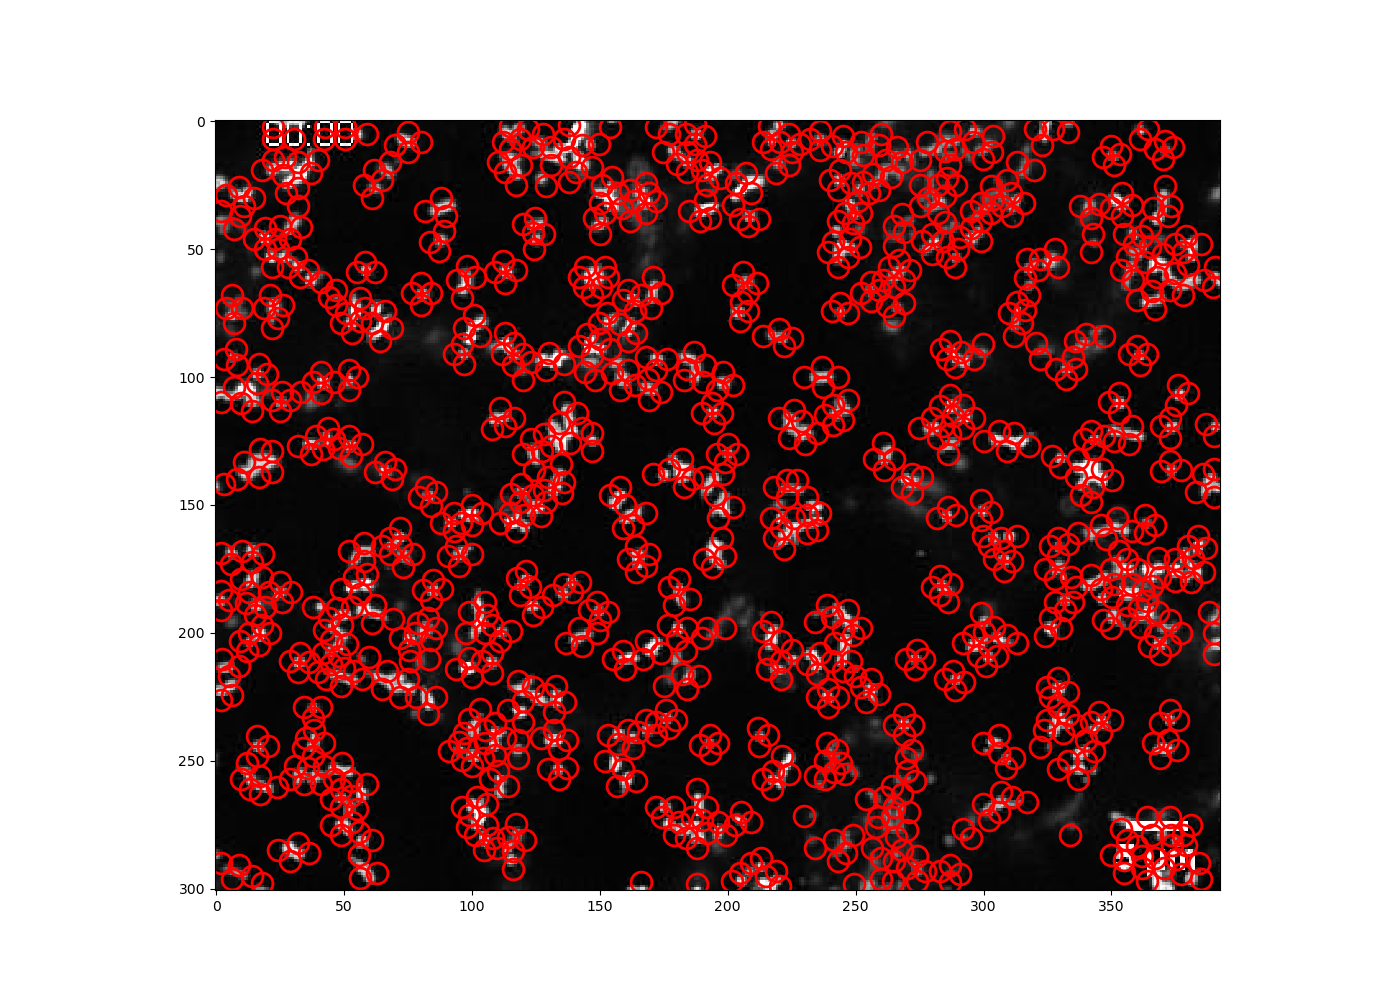
\includegraphics[scale=0.35]{Grafiken/trackpyBilder/locate(f0, diameter=3).png}
    \caption{locate(frames[0], 3)}
    \label{fig:bild_label}
\end{figure} 

Das Bild zeigt eine potente Lokalisierung der Partikel. Es wurde dabei fast alle Elemente des Bildes erkannt, wobei offensichtlich eine deutlich große Menge \textit{false Positive} ist. \\
Eine Verfeinerung der Lokalisierung würde somit einen größeren Durchmesser erfordern. Dies erfolgt in der Folge durch die Verwendung einer immer noch ungeraden Zahl, die jedoch einen größeren Wert hat. In diesem Fall ist es neun, da es so viele "False Positives" gibt. 
\texttt{locate(frames[0], 9)}

\begin{figure}[H]
    \centering
    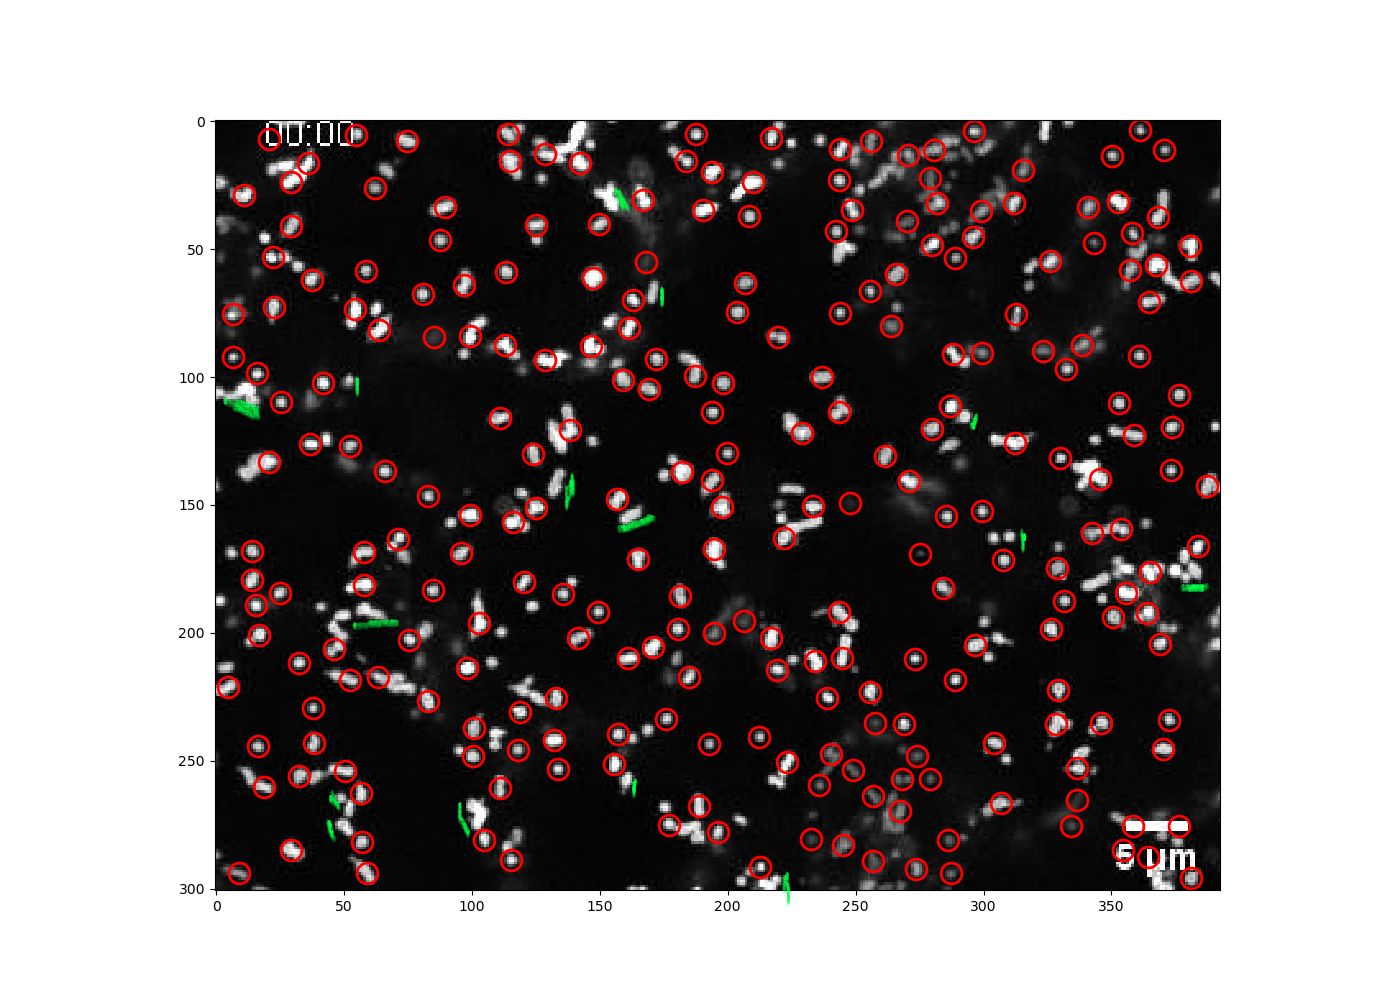
\includegraphics[scale=0.35]{Grafiken/trackpyBilder/locate(frames[0], 9).png}
    \caption{locate(frames[0], 9)}
    \label{fig:bild_label}
\end{figure} 

Diesmal gibt es zwar viel weniger ungewollte Teilchen. Allerdings hat sich eine große Anzahl von "False Negatives" gebildet. \\
Aus diesem Grund wurde nacheinander der Durchmesser von sieben und dann von fünf ausprobiert.\\
\texttt{locate(frames[0], 7)}   gefolgt  \texttt{locate(frames[0], 5)}
\newpage

\begin{figure}[H]
    \centering
    \begin{minipage}{.5\textwidth}
     	\centering
  	  	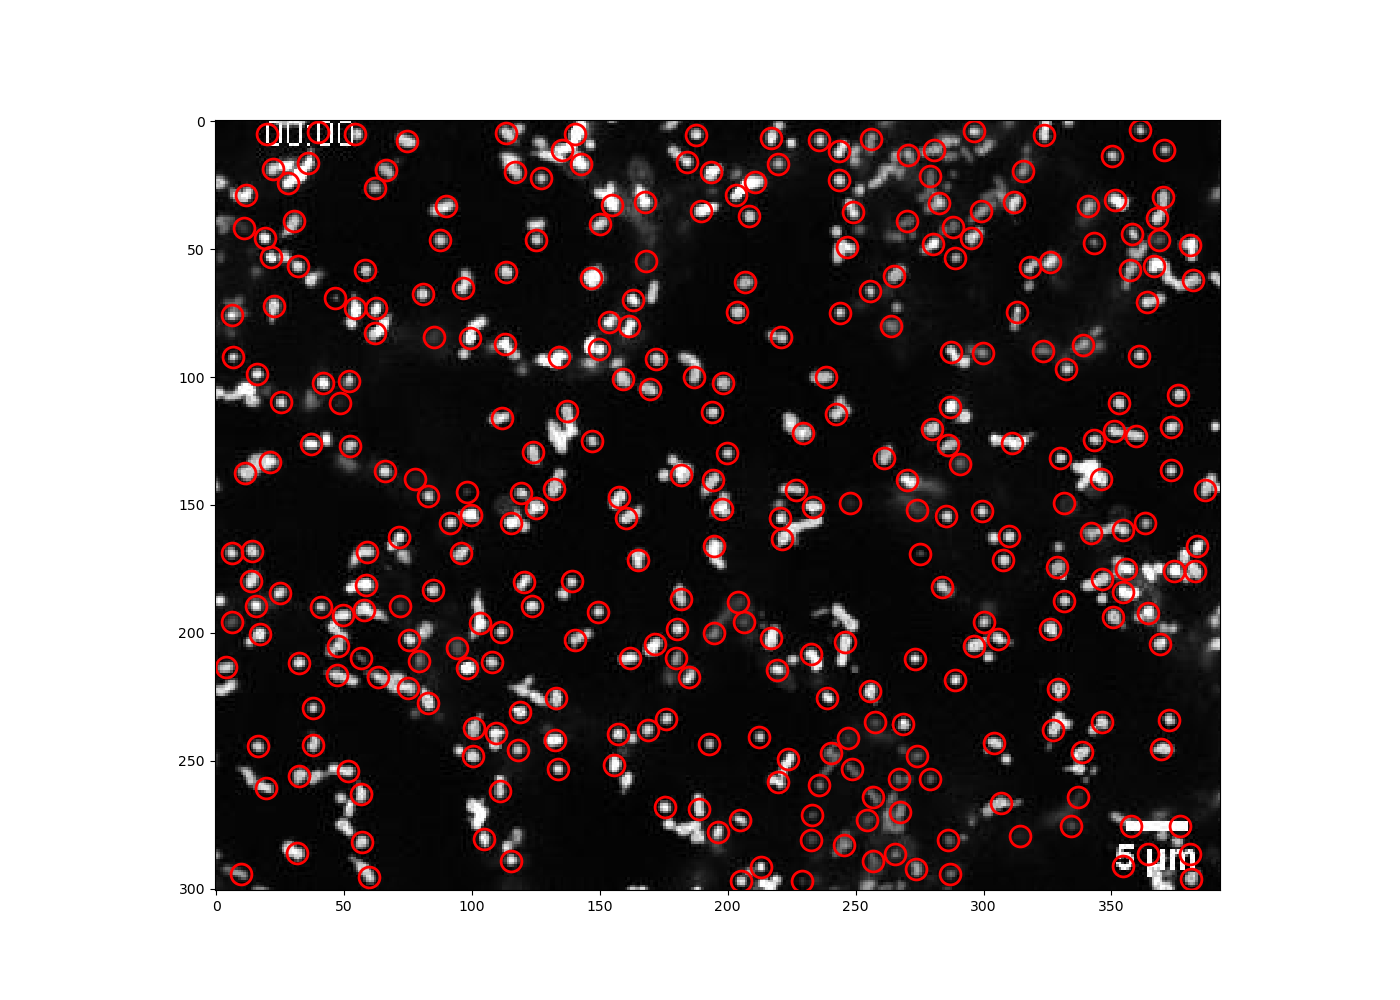
\includegraphics[scale=0.3]{Grafiken/trackpyBilder/locate(frames[0], 7).png}
 	 	\captionof{figure}{locate(frames[0], 7)}
 		\label{fig:test1}
    \end{minipage}
	
	\begin{minipage}{.5\textwidth}
     	\centering
  	  	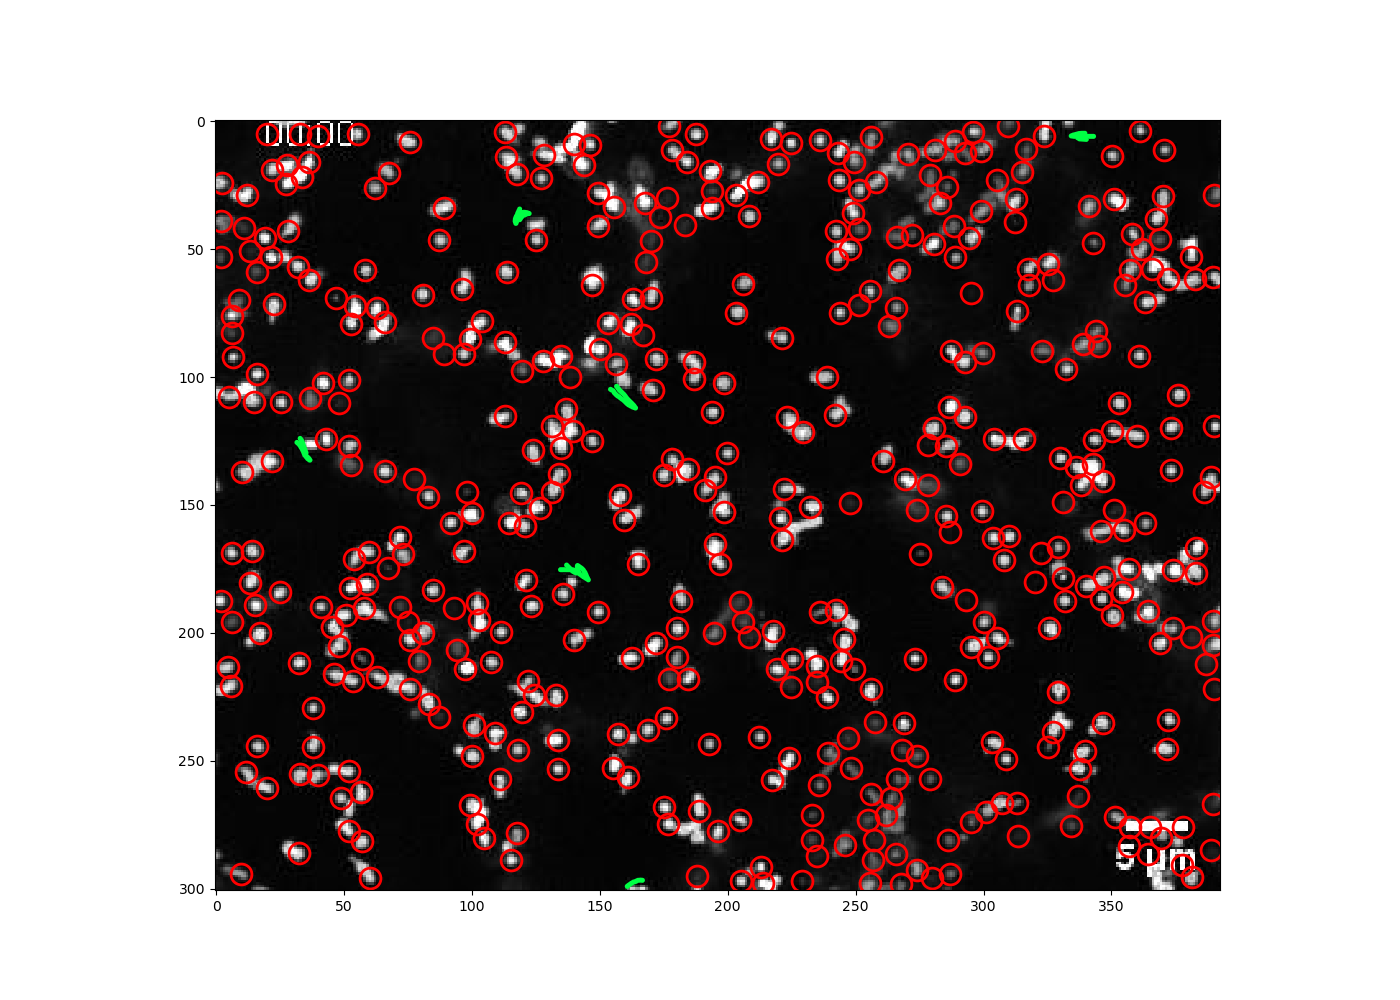
\includegraphics[scale=0.3]{Grafiken/trackpyBilder/locate(frames[0], 5).png}
 	 	\captionof{figure}{locate(frames[0],5)}
 		 \label{fig:test2}
    \end{minipage}
\end{figure}

In Anbetracht des Ziels, einen Durchmesser zu finden, der die Erkennung möglichst vieler Partikel ermöglicht und gleichzeitig möglichst wenig unerwünschte Partikel enthält, ist es besser, mit dem Durchmesser 5 fortzufahren. Denn aus den zuvor verwendeten Durchmessern geht hervor, dass bei diesem Bild die Anzahl der nicht-lokalisierten Teilchen umso größer ist, je höher der Durchmesser ist. 
Dies ist nicht als Allgemeingültigkeit zu verstehen, da verschiedene Videos unterschiedliche Arten von Partikeln mit variierenden Größen und Dicken aufweisen. Es wäre ratsam, die Parameter bei jedem neuen Video zu testen.
Tatsächlich lassen sich insgesamt 475 Partikeln finden, von denen ca. 121 unerwünscht waren und kaum fehlten. Dies entspricht einer ungefähren Rate von 25.47\%.

\begin{figure}[H]
    \centering
    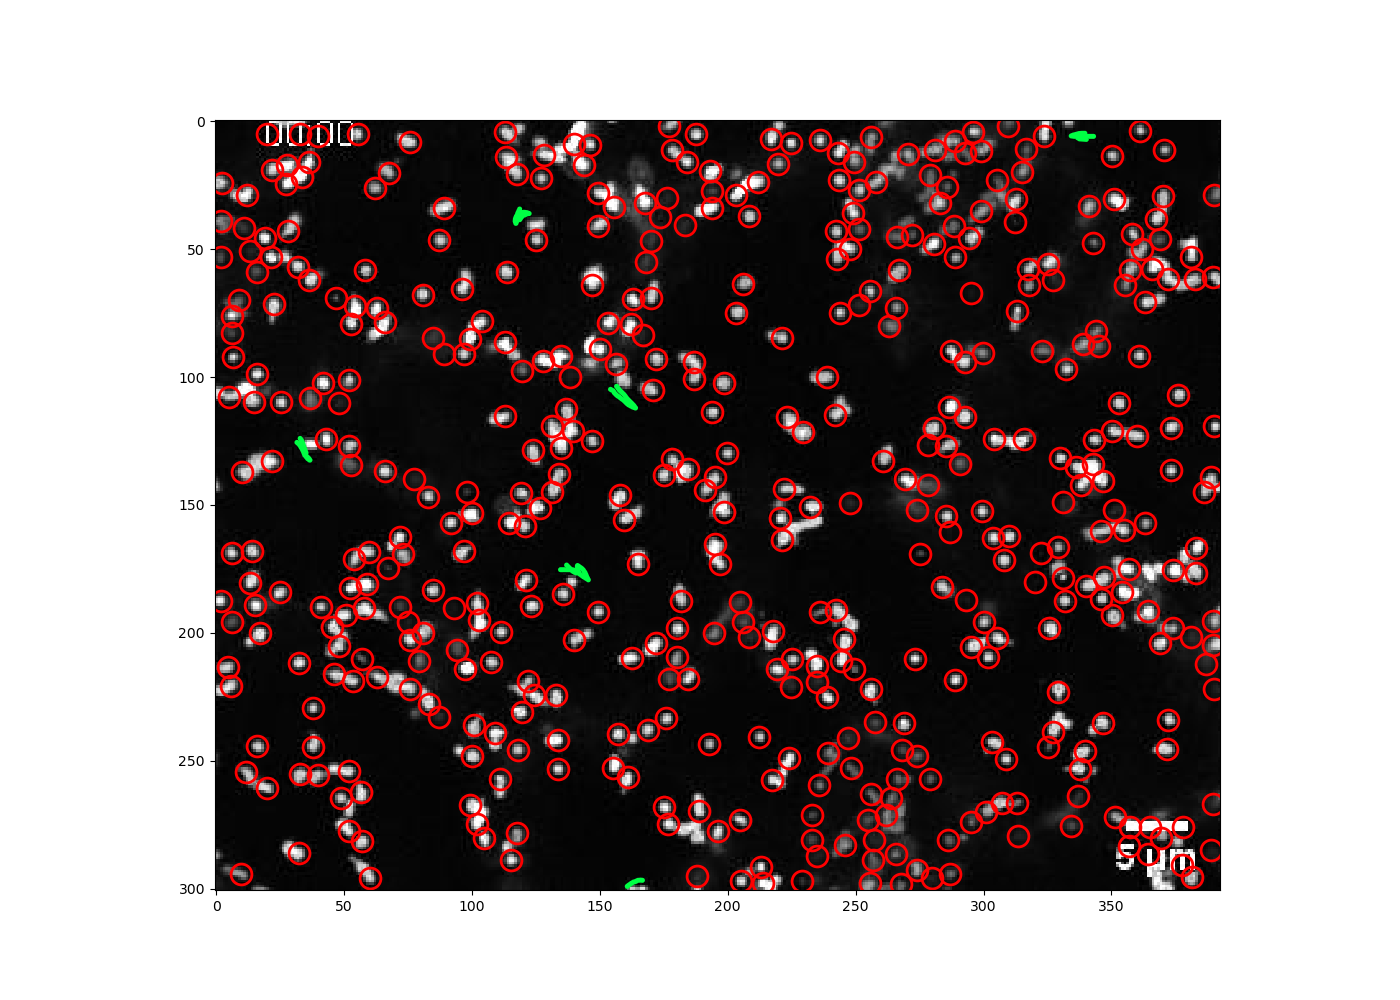
\includegraphics[scale=0.35]{Grafiken/trackpyBilder/locate(frames[0], 5).png}
    \caption{locate(frames[0], 5)}
    \label{fig:bild_label}
\end{figure} 
%    			 In diesem Sinne sieht das Ergebnis der Lokalisierung ohne weitere Parameter wie folgt aus:
%\begin{figure}[H]
%    \centering
%    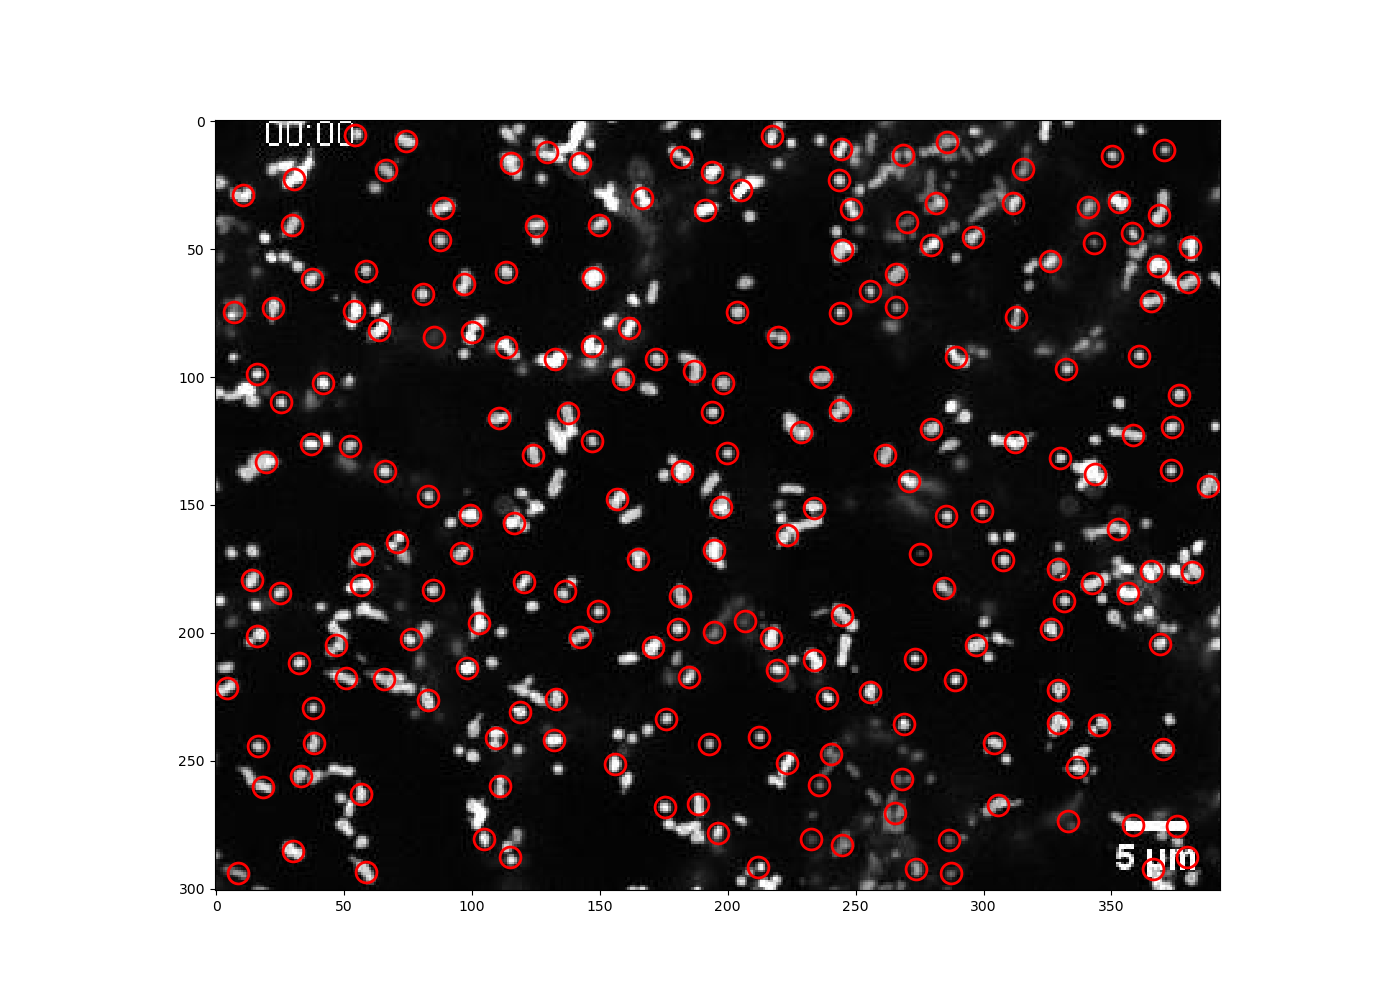
\includegraphics[scale=0.35]{Grafiken/trackpyBilder/locate_with_required_parameter.png}
%    \caption{locate with needed Parameters}
%    \label{fig:bild_label}
%\end{figure}
%    			Wie auf dem \ref{fig:bild_label} zu sehen ist, wurde eine Menge an Partikel 
%    			nicht erkannt, während andere unerwünschten erkannt wurden. 
%    			Insgesamt lassen sich 207 Partikeln finden, von denen 22 unerwünscht waren  und 91 fehlten. Dies entspricht einer ungefähren Rate von 10,628\% für die unerwünschten und einer Rate von 43,9617\% für die nicht gefundenen.

    			
    			\item \textbf{locate(f, d, minmass)}:\\ \\
%    			Da ca. nur 10\% der letzten Suche unerwünschte Elemente waren, wird den Durchschnitt der \textit{minmass} aller Teilchen berechnet und als \textit{minmass} verwendet. Aus der vorherigen \textsc{Panda.Dataframe} genügt es den Mittelwert aus den Werten der \textit{mass}-Spalte zu berechnen, um auf \textit{minmass} von ca. 2490.21 zu gelangen. Das Resultat wird dann wie folgt aussehen:
Wie bereits erwähnt, spiegelt \textit{minmass} die inhärente und eingebaute minimale Helligkeit jedes lokalisierten Partikels wider. Das Ziel ist es nun, die zuvor ermittelten, zu dunklen Partikel herauszufiltern. Daher ist es notwendig, methodisch mit dem Parameter \textit{minmass} zu spielen, um dieses Ziel zu erreichen. Es gibt natürlich mehrere Möglichkeiten, den optimalen Wert für die gesuchte Parameter zu finden. Allerdings wird hier die folgende Logik verfolgt:\\

Aus dem DataFrame der letzten Suche (locate(frames[0], 5)) wurde ja 475 Partikel gefunden. Davon sind ca. 25.47\%, also 121 unerwünscht. Diese Zahl entspricht so fast allen gefundenen zu dunklen Partikel. In anderen Worten, stellt sie die Elemente dar, deren \textit{minmass} zu niedrig ist.
So könnte der Dataframe verwendet werden und ihn nach der Spalte \textit{mass} absteigend sortieren. 
Dies würde dazu führen, dass unsere dunkelsten Partikel am Ende der Liste (Tabelle) positioniert werden und die hellsten ganz oben. Dazu muss keine Funktion implementiert werden, sondern es genügt, die Funktion \textit{sort\_values()} aus der Panda. Dataframe-Bibliothek aufzurufen. Der Aufruf sowie die Tabelle sähe jeweils dann wie folgt aus:\\ \texttt{dataframe.sort\_values(by=['mass'], ascending=False)}

\begin{figure}[H]
    \centering
    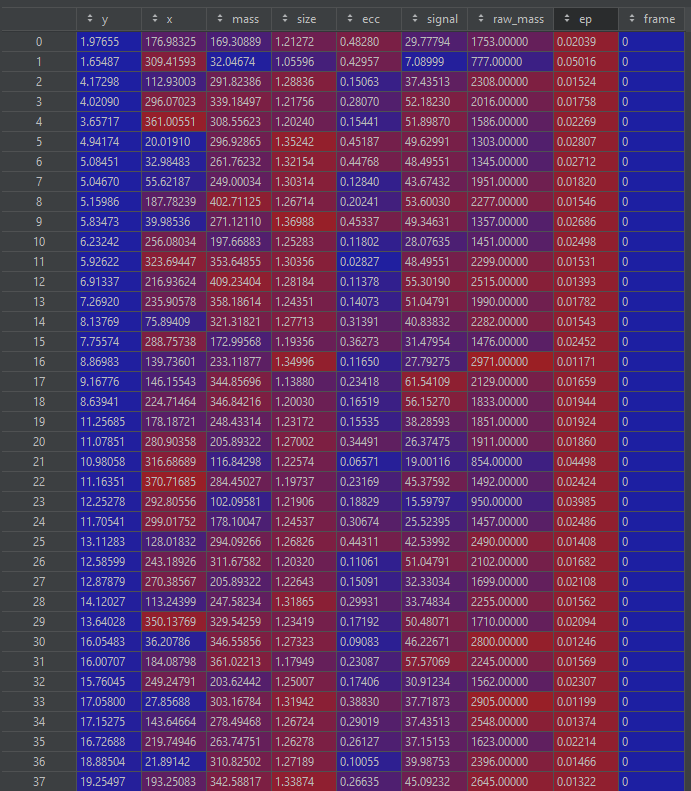
\includegraphics[scale=0.35]{Grafiken/trackpyBilder/df_initial.png}
    \caption{Ein Teil des initialen Dataframes}
    %\label{fig:bild_label}
\end{figure}

\begin{figure}[H]
    \centering
    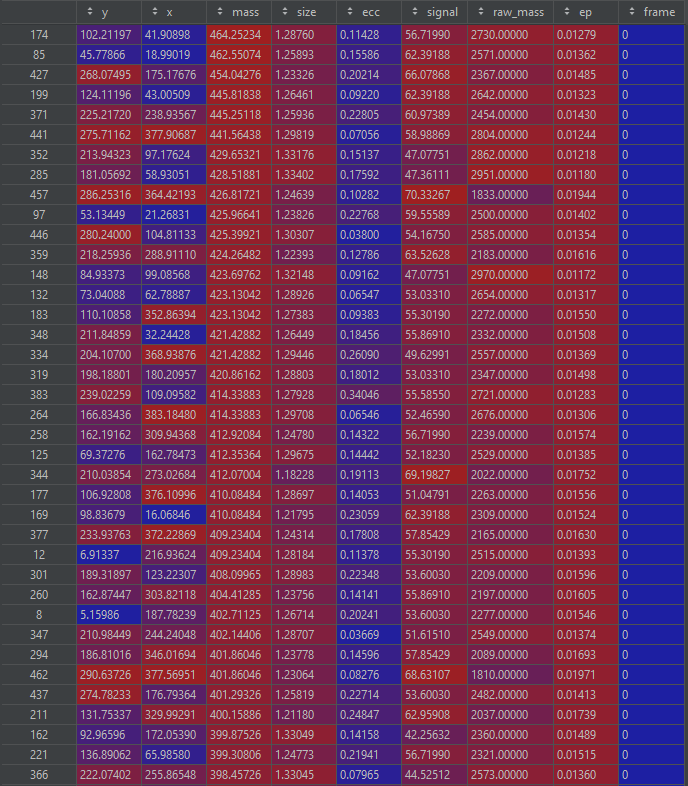
\includegraphics[scale=0.35]{Grafiken/trackpyBilder/df_sorted.png}
    \caption{Ein Teil des sortierten Dataframes}
    %\label{fig:bild_label}
\end{figure}

Jetzt wird es auf dem sortierten Dataframe eine weitere Funktion aufgerufen, um lediglich nur die 354 (also 475-121)gewünschte Partikel bwz. hellsten zu behalten. Eine solche Funktion \textit{head()} wird auch von Panda-Dataframe bereitgestellt. Aus diesem Ergebnis reicht es aus, die von Python angebotene Funktion \textit{min()} auszuführen, um den kleinsten Wert in der Spalte \textit{mass} zu erhalten. 
Die Aufrufe sähen dann wie folgt aus:\\
\texttt{dataframe.head(354)} \\
\texttt{min(dataframe['mass'])}\\

\textbf{189.7280490025089} ist hier das Ergebnis der vorherigen Vorgänge und damit auch den minimalen Wert von \textit{mass}, den ein Partikel haben muss. Es sei der \textit{minmass} Parameter der Funktion \textit{locate()}.



%Es wurde zwar fast alle \textit{False Positive} beseitigt, aber dafür wurde eine viel zu hohe Anzahl an \textit{True Negative} nicht gefunden. Die Lösung für dieses Problem besteht darin, den Wert von "minmass"  schrittweise zu verringern, bis ein zufriedenstellendes Ergebnis erzielt wird.
\begin{figure}[H]
    \centering
    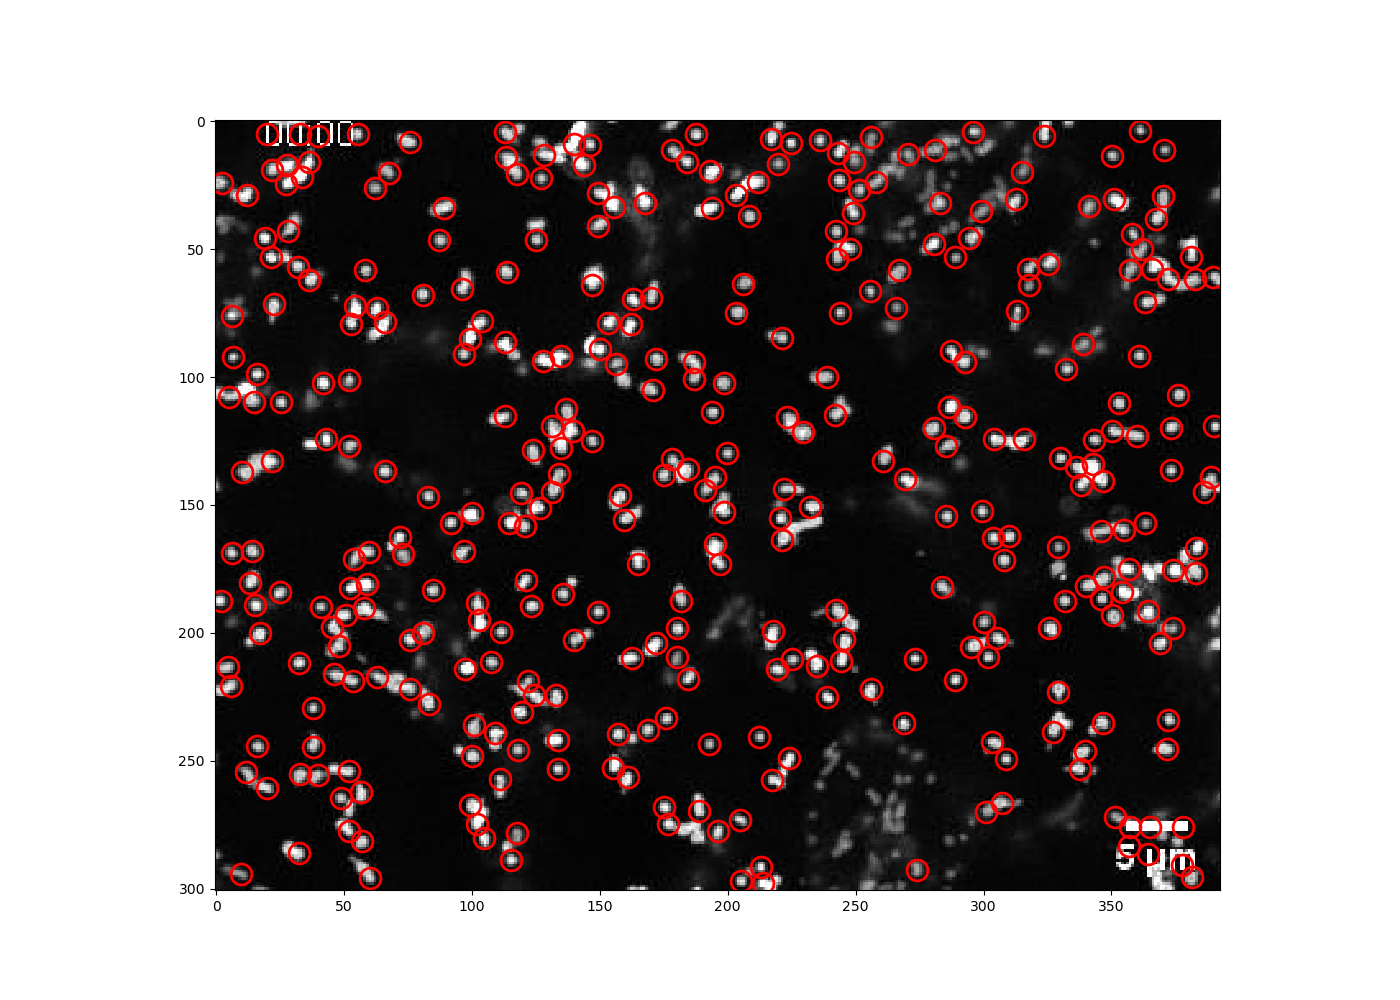
\includegraphics[scale=0.35]{Grafiken/trackpyBilder/locate_with_minmass_01.png}
    \caption{locate with 'mimass=189.7280490025089'}
    %\label{fig:bild_label}
\end{figure}

		\item locate(frames[0], 11, minmass=1000.0, separation=2, noise\_size=1.5): \\ \\
    			Hier wird es einfach Werte bei \textit{separtion} und \textit{noise\_size} ausprobiert, um auf die bessere Resultate zu kommen. Dies ergibt in diesem Fall:
    			
\begin{figure}[H]
    \centering
    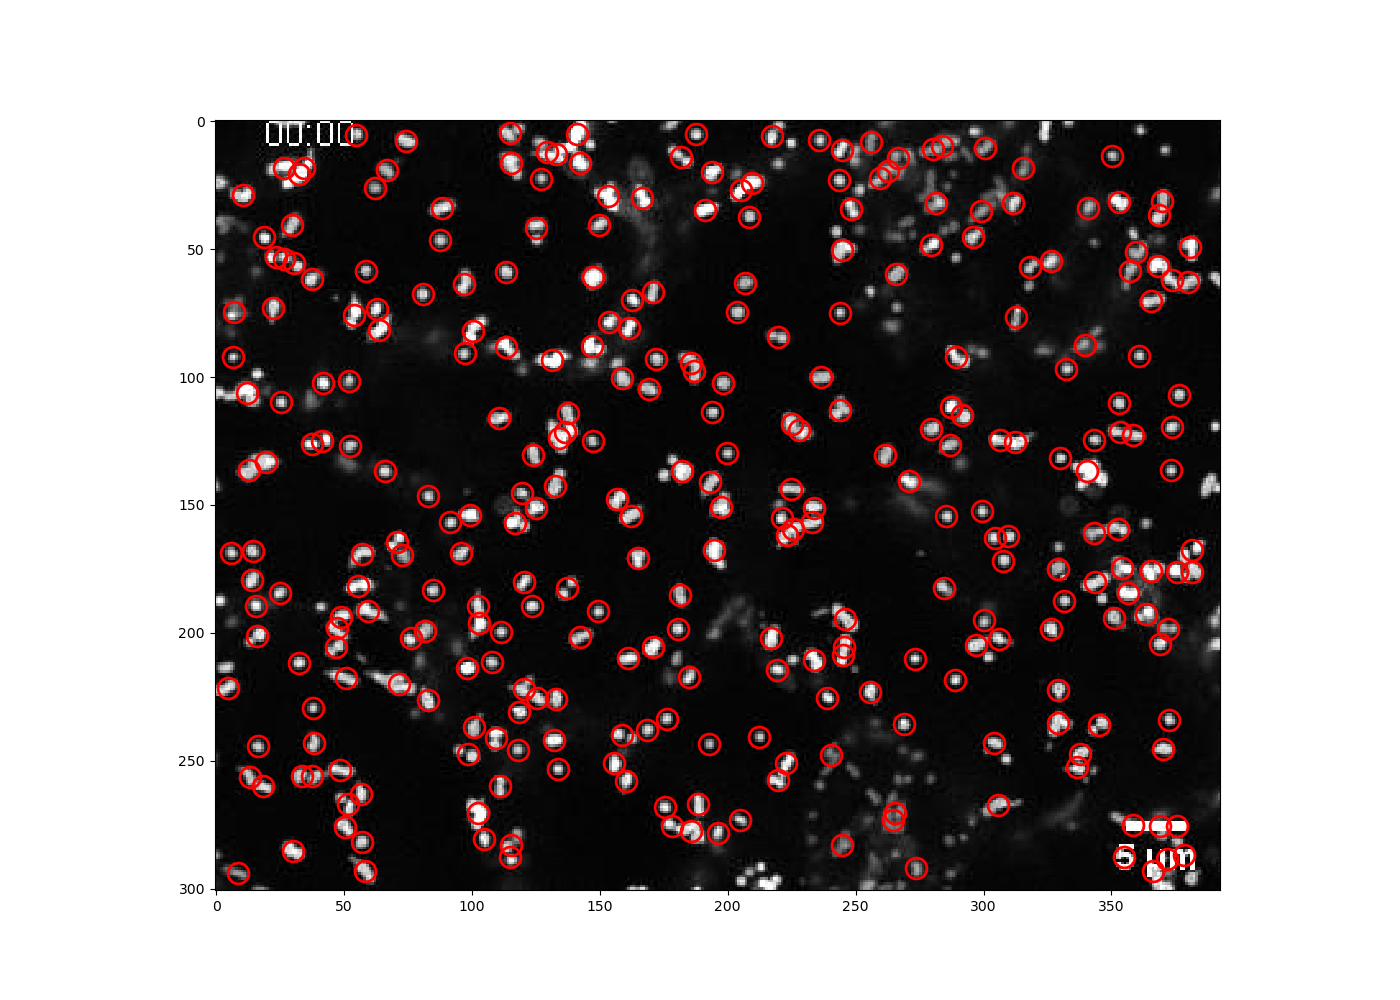
\includegraphics[scale=0.35]{Grafiken/trackpyBilder/locate_with_separation__noise_size.png}
    \caption{locate with 'sep=3.0 and n\_s=1.5'}
    %\label{fig:bild_label}
\end{figure}


\item locate(frames[0], 11, minmass=1000.0, separation=2, noise\_size=1.5, topn=250):    \\ \\ 
		Nachdem alle vorherige Parameter eingesetzt worden sind, wenn der Dataframe immer noch sanierungsbedürftig ist, wird auch \textit{topn} zum Einsatz gebracht. Dazu wird die Anzahl an bestehende unerwünschte Elemente geschätzt und von der gesamten Anzahl an gefundenen Elemente abgezogen. Somit wird \textit{topn} in dem Fall hier auf \textit{250} geschätzt. (siehe Bild)
\begin{figure}[H]
    \centering
    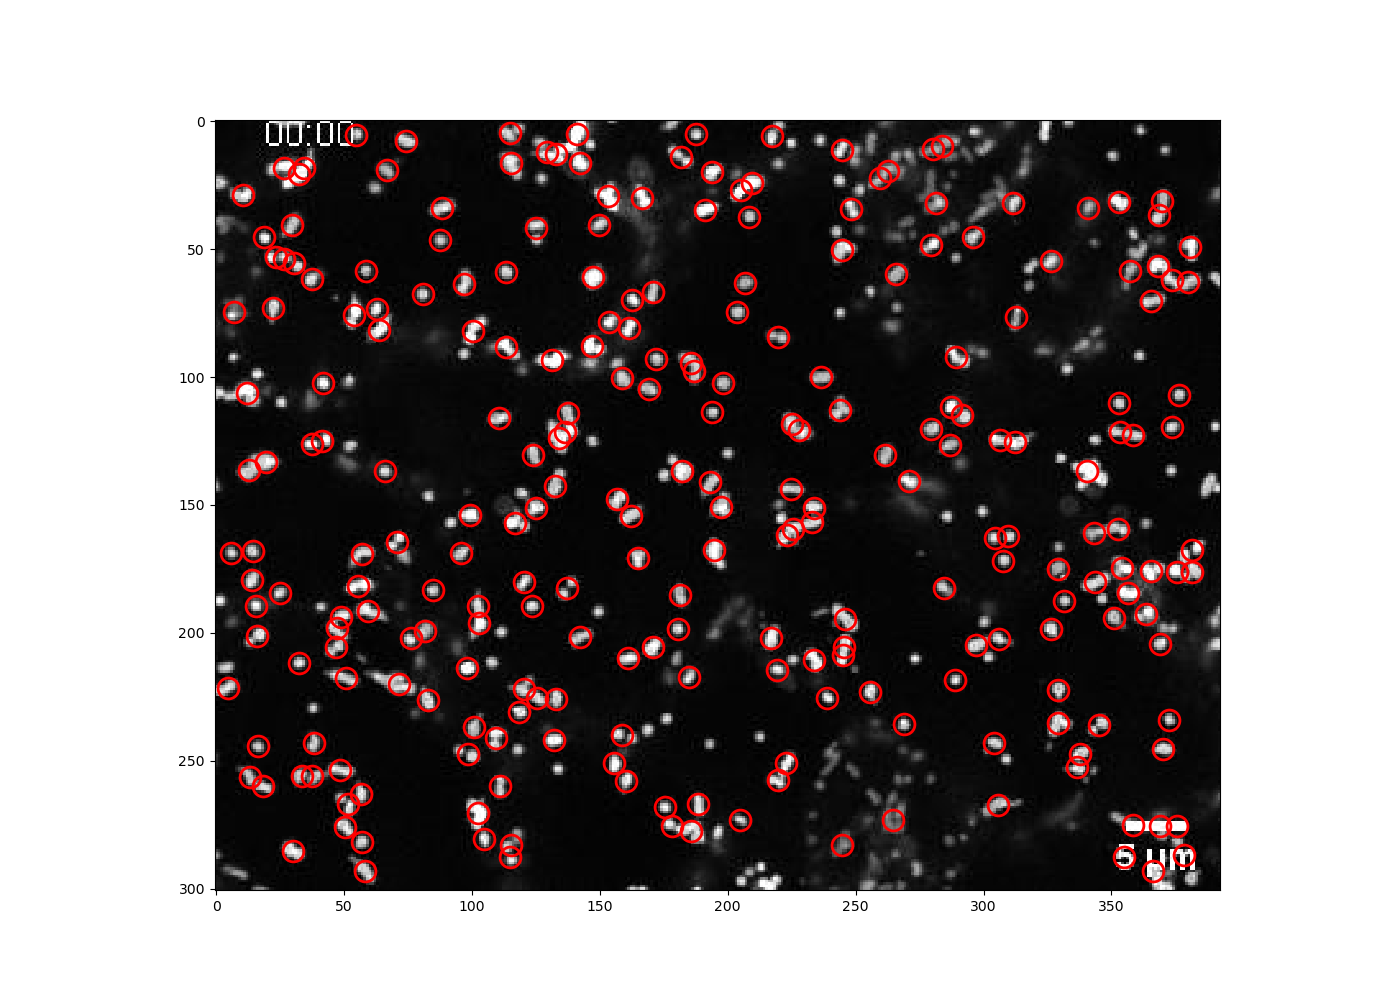
\includegraphics[scale=0.35]{Grafiken/trackpyBilder/locate_with_topn.png}
    \caption{locate with 'topn=250'}
    %\label{fig:bild_label}
\end{figure}
\end{enumerate}
\subsection{Machine Learning}



%\addcontentsline{toc}{chapter}{Kapitel-2}
\chapter{Trackpy \label{kap2}}

Dieser Arbeitsteil  wird sich hauptsächlich mit einer Einführung in die Software beschäftigen. Des Weiteren wird es um ihre Installation und die Erfahrungen des Nutzers mit der Software gehen.

%\addcontentsline{toc}{section}{Kapitel-2}
\section{Einleitung und Installation \label{Kap2.1_Einleitung_Installation}}
Trackpy ist ein Python-Paket, das, wie im Abschnitt \ref{kap1_trackpy} beschrieben, nicht nur Informationen über die Partikel in einem Video (sowohl in hoher als auch in niedriger Auflösung) liefert, sondern auch mit ihnen interagieren (wie zum Beispiel einen Trajektorie der XY-Koordinaten zu zeichnen, die ein Partikel während der Aufnahmen erreicht hat.) kann, und zwar sowohl in 2D als auch in 3D. Das Programm verfügt über eine gut durchdachte Dokumentation, die die Installation und das Eintauchen in das Programm erleichtert.
Aus diesem Grund werden wir uns bei der Installation nur auf die auf der Website \cite{tp_installation} angegebenen Schritte stützen und eventuell weitere Schritte erwähnen, die nicht angegeben wurden.\\
Nachdem alle Schritte befolgt wurden, sollte die Installation ohne Probleme abgeschlossen werden können. Die Nutzung der Bibliothek verläuft jedoch noch nicht ganz so, wie im Benutzerhandbuch beschrieben. Daher werden die Unterschiede in der Nutzung im Abschnitt \ref{kap2.2_benutzererfahrung} behandelt.


\section{Benutzererfahrung \label{kap2.2_benutzererfahrung}}

\subsection{In Bezug auf das Lesen des Videos \label{kap2.2.a_lesen_video}}
Die Bibliothek verspricht eine problemlose Ablesung verschiedener Videoformate wie \textit{AVI}, \textit{h.264}, \textit{Tiff-Stacks} und viele andere, indem man einfach die Funktion \textit{open()} oder \textit{video()} aus der \textbf{PIMS}-Bibliothek \cite{pims} verwendet. Leider erfordert das Abspielen von Videos hier die Installation einer beliebigen Bibliothek, die das Abspielen von Videos ermöglicht. In unserem Fall haben wir also \textbf{ffmpeg} und \textbf{scikit-image} verwendet.\\
Um dies zu tun, müssen diese beiden ebenfalls installiert werden. Wenn Pycharm wie empfohlen als IDE verwendet wird, muss die Installation folgendermaßen durchgeführt werden:  \textbf{STRG$+$ALT$+$S} drücken, dann \textit{Interperter} in die Suchleiste eingeben und  auf \textit{Python Interpreter} klicken. 
Auf der rechten Seite des Fensters erscheint dann eine Liste der installierten Pakete. Jetzt muss man auf die Schaltfläche $+$ klicken, um die zu installierenden Pakete zu finden, und dann auf \textit{Installieren} klicken.\\
Sicherheitshalber sollten Sie auch darauf achten, dass \textit{trackpy}, \textit{bokeh}, \textit{ffmpeg} und \textit{scikit-image} in der Liste der bereits installierten Pakete enthalten sind. 

\subsection{In Bezug auf die Einarbeitung in die Bibliothek \label{kap2.2.b_einarbeitung}}

Das Eintauchen und Einarbeiten in diese Bibliothek wird durch die Präsenz eines "\textbf{Walkthrough}''  auf der Website sehr erleichtert.  In diesem \textit{Walkthrough} geht es vor allem um die grundlegende Nutzung fast aller wichtigsten Funktionen dieser Bibliothek anhand eines praktischen Beispiels, das Schritt für Schritt zeigt, wie man zu den Ergebnissen gelangt, die mit Bildern illustriert sind.\\
Dies ermöglichte uns einen leichten Einstieg und eine schnelle Nutzung der benötigten Funktionen. Abgesehen von der Wiedergabe von Videos, wie sie im Abschnitt  \ref{kap2.2.a_lesen_video} beschrieben ist.


\subsection{In Bezug auf die Geschwindigkeit \label{kap2.2.c_geschwindigkeit}}
Was die Ausführungsgeschwindigkeit betrifft, finden wir, dass sie für die Informationen, die sie über die vorhandenen Partikel liefert, recht schnell ist.  Wir sprechen hier in den meisten Fällen von wenigen Sekunden. \\
Bei zusätzlichem Bedarf an Leistung (Geschwindigkeit) gibt es auf ihrer Website auch eine Anleitung, wie man Trackpy noch schneller machen kann.

\newpage

\subsection{In Bezug auf Verwendung bestimmter Parameter der Funktion locate. \label{kap2.2.d_verwendung_locate_param}}
Tatsächlich gibt es zwar eine Dokumentation von fast allen Anwendungsfällen von Trackpy. Insbesondere hier bei den Parametern der Funktion "\textit{locate()}" gibt es eine Reihe von Parametern, die nicht so funktionieren, wie in der Dokumentation beschrieben. 
Die meisten von ihnen sind in diesem Abschnitt \ref{non_working_param} zu finden. 
Aber um unsere Aussagen hier zu verdeutlichen, nehmen wir einen dieser Parameter, die nicht funktionieren, nämlich:

\begin{itemize} 
	\item \textbf{max\_iterations}: soll das Ergebnis der Erkennung in jeder Schleife verfeinern. Das Standardwert ist 10, egal welcher Wert zugewiesen wird, größer als 0, es gibt keinen sichtbaren Unterschied (siehe \ref{fig:comparison max-iterations}). 
	\begin{figure}[H]
    \centering
    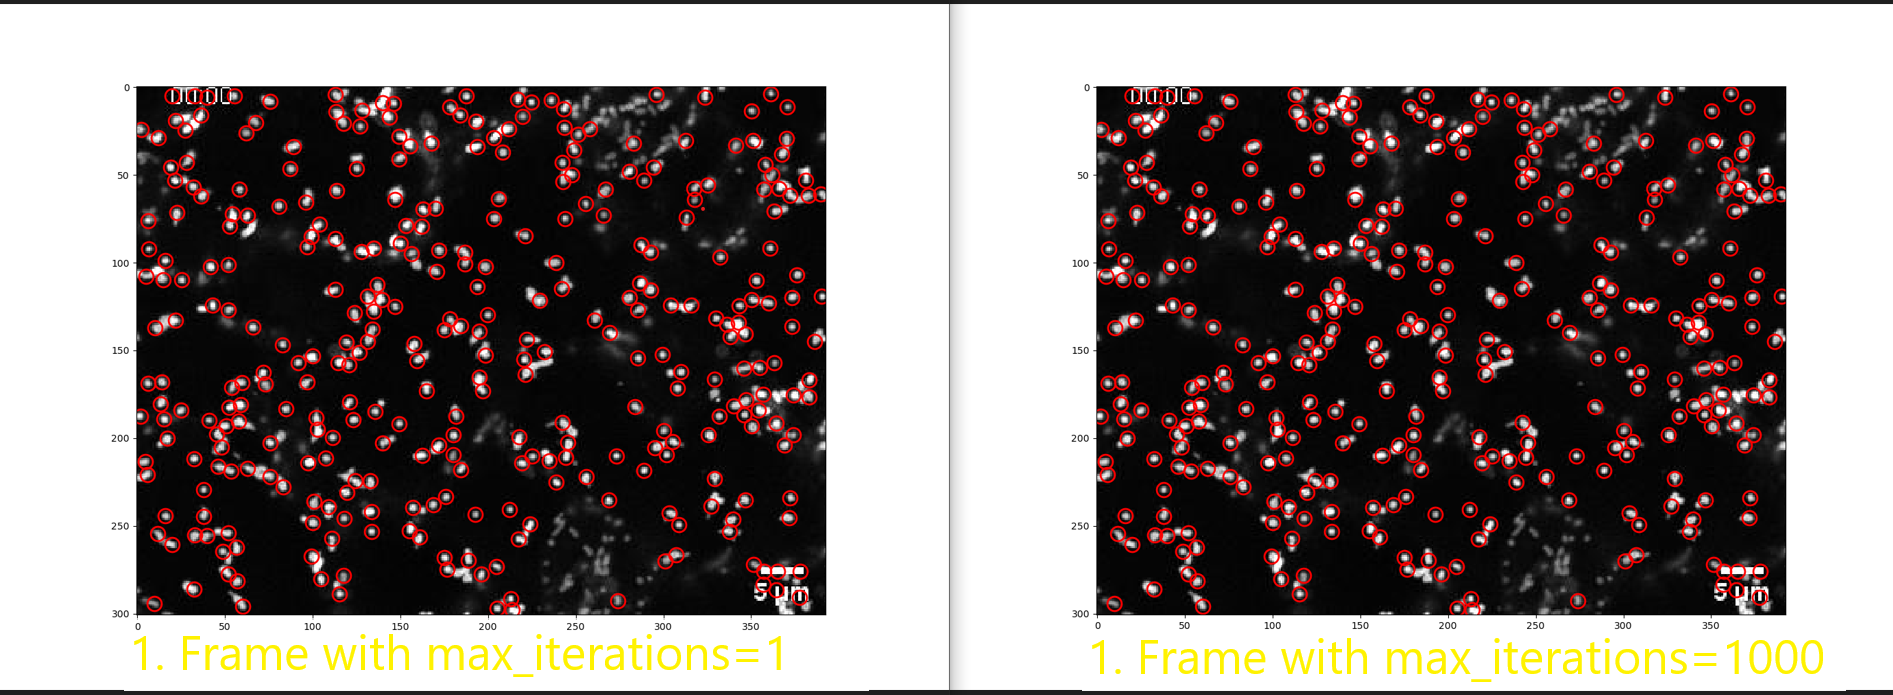
\includegraphics[scale=0.35]{Grafiken/trackpyBilder/comparison max_iterations.png}
    \caption{Vergleich zwischen max\_iterations=1 und max\_iterations=1000 auf demselben Frame.}
    \label{fig:comparison max-iterations}
\end{figure} 
	
\end{itemize}

%\addcontentsline{toc}{chapter}{Kapitel 3}
\chapter{Partikel-Erkenung-System \label{kap3}}

%\addcontentsline{toc}{section}{Kapitel 3}
\section{Partikel-Erkenung-System}
PES (Partikel-Erkenung-System)  ist eine Software, die wir im Rahmen dieser Arbeit entwickelt haben und die es ermöglichen soll, die in einem Bild vorhandenen Partikel zu lokalisieren und auch die Ergebnisse zu bewerten, indem die den Parametern zugewiesenen Werte verglichen werden. 
Um die Partikel zu lokalisieren, verwendet das PES ausschließlich die Bibliothek trackpy, die es ihm mit ihrer Funktion "locate" ermöglicht, die Partikel zu erkennen.\\
Im Folgenden werden wir die verschiedenen Parameter dieser Funktion vorstellen, die nach unserer Einschätzung der Effektivität und Wichtigkeit in zwei Gruppen eingeteilt sind.
	\subsection{Parameter der locate-Funktion \label{kap3_param_loacate}}
		Folgende Parameter werden im Laufe dieser Arbeit angewandt:

		\begin{enumerate}
    			\item raw\_image: array of images \\
    			Wird für die endgültige Charakterisierung verwendet.
    			
    			\item diameter: odd integer \\
    			Entspricht der geschätzten Größe der Partikeln (in Pixel). Es wurde leider kein Grund für die Verwendung einer ungeraden Zahl angegeben.
    			\item minmass: float \\
    			Minimale eingebaute Helligkeit. Dies ist ein Schlüsselparameter, um störende 				Merkmale zu entfernen. Der Standardwert ist es 'None'.\\
    			\label{none}None ist ein Typ in Python, der es ermöglicht, einer Variablen keinen festen Wert zuzuweisen. Da minmass optional ist, würde None gewählt, damit der Wert nicht direkt mit der Partikelerkennung interferiert. Und None ist eine gute Möglichkeit, dies in Python zu tun.
    			
    			\item maxsize: float\\
    			Maximaler Gyrationsradius der Helligkeit.\\
    			Wobei der Gyrationsradius \cite{raduis_of_gyration} definiert den Abstand von der Rotationsachse zu dem Punkt, an dem die gesamte Masse eines Körpers konzentriert sein soll, der das gleiche Trägheitsmoment wie die ursprüngliche Form aufweisen soll.    			
    			
    			\item separation: float\\
    			Minimaler Abstand zwischen den Partikeln. Der Standardwert ist \textit{diameter + 1}.\\
    			Natürlich können auch negative Werte angegeben werden, aber das würde das Ergebnis nur verfälschen. Wie in dem Punkt, in dem es um die richtige Wahl für die Separation geht, erwähnt, führt jeder Wert unterhalb des Diameters nur zu einer Vervielfachung der Anzahl der erkannten Partikel, obwohl es sich um dieselben Partikel handelt, die sich an denselben Positionen befinden.			
    			
    			\item noise\_size: float or tuple\\
    			Breite des Gaußschen Weichzeichner-kerns, in Pixeln. Der Standardwert ist 1.\\
    			Wobei  ein Gaußscher Weichzeichner ist nichts anderes als die Anwendung einer mathematischen Funktion auf ein Bild, um es weichzuzeichnen.
    			
    			\item topn: interger\\
    			Gibt lediglich die N hellsten Merkmale über minmass zurück. Wenn 'None' (Voreinstellung), werden sämtliche Eigenschaften oberhalb von minmass zurückgegeben. \\
    			Die Wahl von 'None' als Standardwert ist hier nichts anderes als derselbe Wert, der auch in \ref{none} erwähnt wird.
    			
    			
		\end{enumerate}
		
Neben diesen Parametern, die wir im Laufe unserer Arbeit verwenden werden, gibt es noch andere, die ebenfalls von trackpy zur Verfügung gestellt werden. Sie sind jedoch aus Gründen der Nützlichkeit oder Funktionsfähigkeit nicht aufgelistet. Im Folgenden werden diese Parameter aufgelistet:

\begin{itemize}\label{non_working_param}
				\item smoothing\_size: float or tuple\\
				Die Größe der Seiten des quadratischen Kerns, der bei der Glättung verwendet wird, in Pixeln. Der Standardwert ist der \textit{diameter}.
				
				\item threshold: float\\
				Schneidet das Ergebnis des Bandpasses unterhalb dieses Wertes ab. Die Schwellwertbildung wird auf das Bild angewendet, das bereits vom Hintergrund subtrahiert wurde. Standardmäßig 1 für Vollbilder und 1/255 für schwebende Bilder.
				
				\item invert: boolean\\
				Auf True gesetzt, wenn die Merkmale dunkler als der Hintergrund sind. Standardmäßig False.
				Dies wird deprecated. Es sollte stattdessen eine geeignete PIMS-Pipeline verwenden, um ein Bild oder eine Sequenz von Bildern zu invertieren.
				
				
				\item percentile: float\\
				Die Merkmale sollten eine hellere Spitze haben als die Pixel in diesem Perzentil. Dadurch werden störende Peaks eliminiert.
				
				\item preprocess: boolean\\
    			Setze auf False, um die Bandpass-Vorverarbeitung zu deaktivieren.
    			
				\item max\_iterations: integer\\
    			Maximale Anzahl der Schleifen zur Verfeinerung des Massenschwerpunkts, Standardwert 10. Er muss immer mindestens größer als 0 sein. Für den Fall, dass wir ihn verwenden wollen.
    			
				\item filter\_before: boolean\\
				Es wird nicht mehr unterstützt, da es die Leistung nicht verbessert.
				
    			\item filter\_after: boolean\\
    			Diese Einstellung wurde deprecated: Verwende stattdessen minmass und maxsize.
    			
    			\item characterize: boolean\\
    			Berechnet die "Extras": Exzentrizität, Signal, ep. Standardmäßig wahr.
    			
    			\item engine: {‘auto’, ‘python’, ‘numba’}\\
    			Bestimmt, mit welchem Compiler die Funktion ausgeführt werden soll.			

\end{itemize}
    					
		
Ein \textsc{Panda.Dataframe} mit den Daten \textit{y-koordinaten, x-koordinaten, mass, size, ecc, signal, raw\_mass, ep, frame} wird als Rückgabewert zurückgegeben. Dies gilt für jedes der gefundenen Partikel (Siehe \ref{fig:kap3_initDataframe}).
Ausführlichere Informationen zu  weiteren Parametern sowie zu den Obengennanten ist auf \cite{Tp} zu sehen.%~ \citep{Tp}% zu sehen. 
An dieser Stelle kann folgende Frage aufgeworfen werden: Was sind die besten Parameterwerte? \\
Beachte, dass einfachheitshalber, während der gesamten Parametereinstellung nur das erste Bild unseres Videos betrachtet wird.

	\subsection{Ermittlung der optimalen Parameterwerte der Locate-Funktion von Trackpy. \label{kap3_OP}}
	Hier wird es ein Antwortversuch auf die zuletzt gestellte Frage eingegangen. Zur Erreichung dieses Zieles wird mit der Erkennung begonnen, indem nur die geforderten Parameter(raw\_image und diameter) verwendet werden und nach und nach weitere hinzugefügt werden, um die Suche zu verfeinern. 
	
	\begin{enumerate}
    			\item {\large \textbf{Ermittlung von diameter}}\\
    			\textbf{locate(f, d): \textit{Wobei f = raw\_image und d = diameter}} \\ \\
    			 Während frames[0] entspricht in diesem Fall dem ersten Bild der Videoaufnahme bzw. der Imagesequenz. \texttt{frames} hingegen bilden die Gesamtheit der Bilder des Videos im Laufe der Zeit und damit die Sequenz der Bilder.  Diese Angabe, die vom Typ Array ist, stellt eine Voraussetzung für die Ausführung von Funktionen dar. \\
    			 Für den Durchmesser wird zunächst willkürlich eine ziemlich kleine ungerade Zahl genommen, um die Ergebnisse zu sehen und eine Annäherung an den Wert, den wir verwenden sollen, zu erhalten. Zunächst nehmen wir also einen Durchmesser von drei (d=3).  
    			 
\begin{figure}[H]
    \centering
    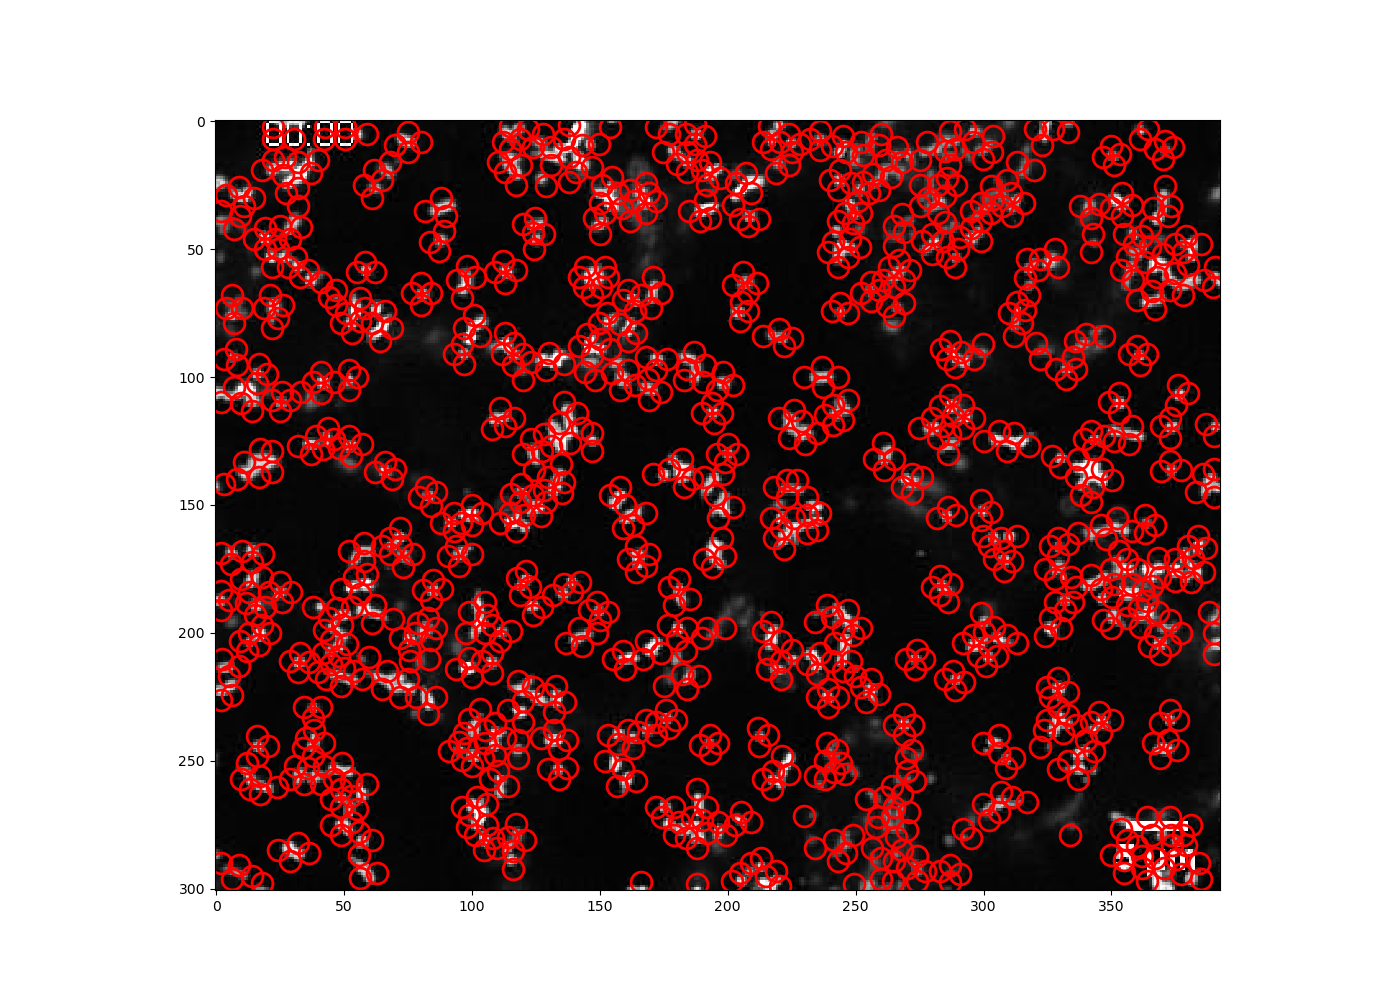
\includegraphics[scale=0.35]{Grafiken/trackpyBilder/locate(f0, diameter=3).png}
    \caption{locate()-Funktion auf 0. Frame mit diameter=3}
    \label{fig:kap3_d=3}
\end{figure} 

Das Bild zeigt eine Lokalisierung der Partikel. Es wurde dabei fast alle Elemente des Bildes erkannt, wobei offensichtlich eine deutlich große Menge \textit{\gls{false positive}} ist.\\
In grüner Farbe haben wir auf dem Bild einige Beispiele für \textit{false Positive} Ergebnisse markiert. 
Hier liegt ein \textit{false Positive} Befund vor, wenn ein Partikel entdeckt wird, das nicht hätte entdeckt werden dürfen. Denn entweder sind sie zu klein, zu dunkel oder sogar zu viele Detektionskreise um das gleiche Partikel.  
\\
Eine Verfeinerung der Lokalisierung würde somit einen größeren Durchmesser erfordern. Dies erfolgt in der Folge durch die Verwendung einer immer noch ungeraden Zahl, die jedoch einen größeren Wert hat. In diesem Fall ist es neun, da es so viele \textit{False Positives} gibt. 
\texttt{locate(frames[0], 9)}

\begin{figure}[H]
    \centering
    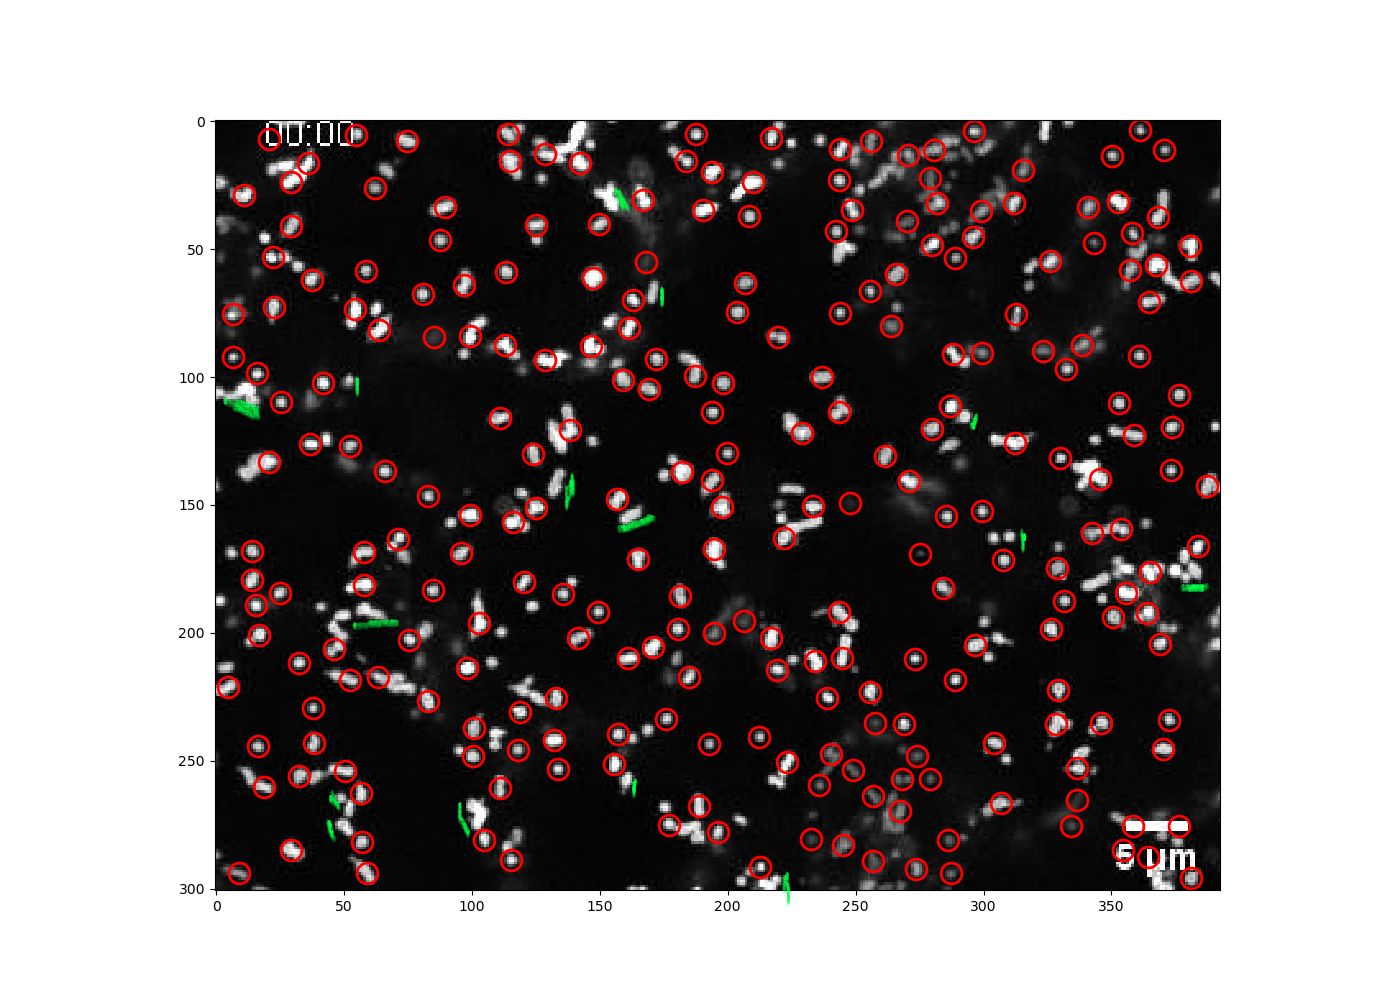
\includegraphics[scale=0.35]{Grafiken/trackpyBilder/locate(frames[0], 9).png}
    \caption{locate()-Funktion auf 0. Frame mit diameter=9}
    \label{fig:kap3_d=9}
\end{figure} 

Diesmal gibt es viel weniger ungewollte Teilchen. Allerdings hat sich eine große Anzahl von \textit{\gls{false negative}} gebildet. \\ 
Auch hier sind auf dem Bild paar Beispiele von  \textit{false Negative} Ergebnisse in grün markiert.
Hier spricht man von \textit{False Negative} Befund, wenn ein Partikel nicht entdeckt wird, das hätte entdeckt werden müssen.
Aus diesem Grund wurde nacheinander der Durchmesser von sieben und dann von fünf ausprobiert.\\
\texttt{locate(frames[0], 7)}   gefolgt  \texttt{locate(frames[0], 5)}
\newpage

\begin{figure}[H]
    \centering
    \begin{minipage}{.5\textwidth}
     	\centering
  	  	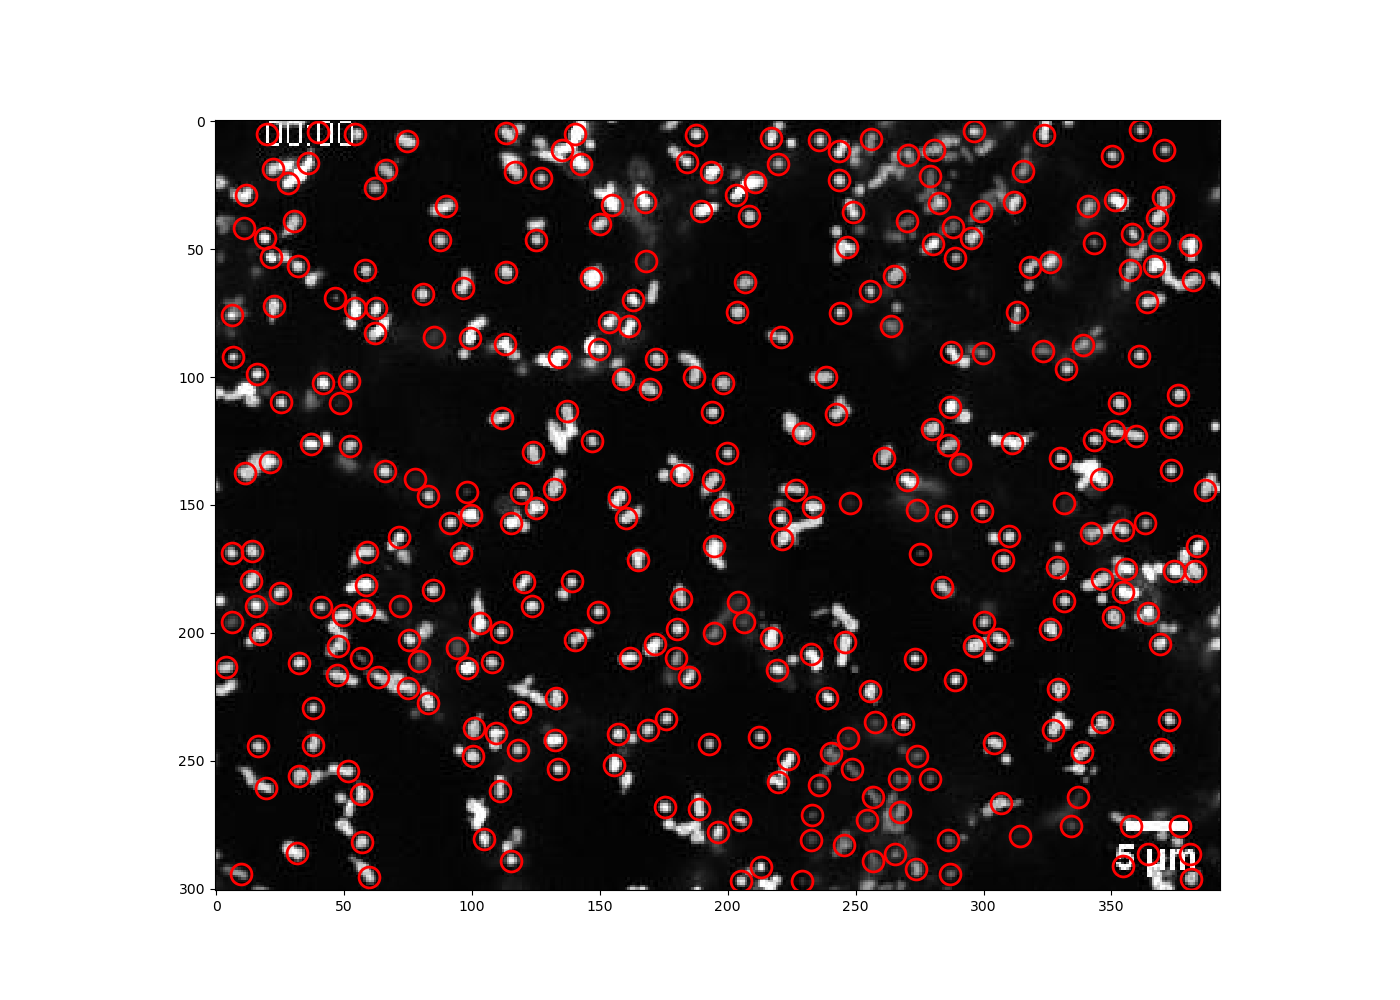
\includegraphics[scale=0.3]{Grafiken/trackpyBilder/locate(frames[0], 7).png}
 	 	\captionof{figure}{locate()-Funktion auf 0. Frame mit diameter=7}
 		\label{fig:kap3_d=7}
    \end{minipage}
	
	\begin{minipage}{.5\textwidth}
     	\centering
  	  	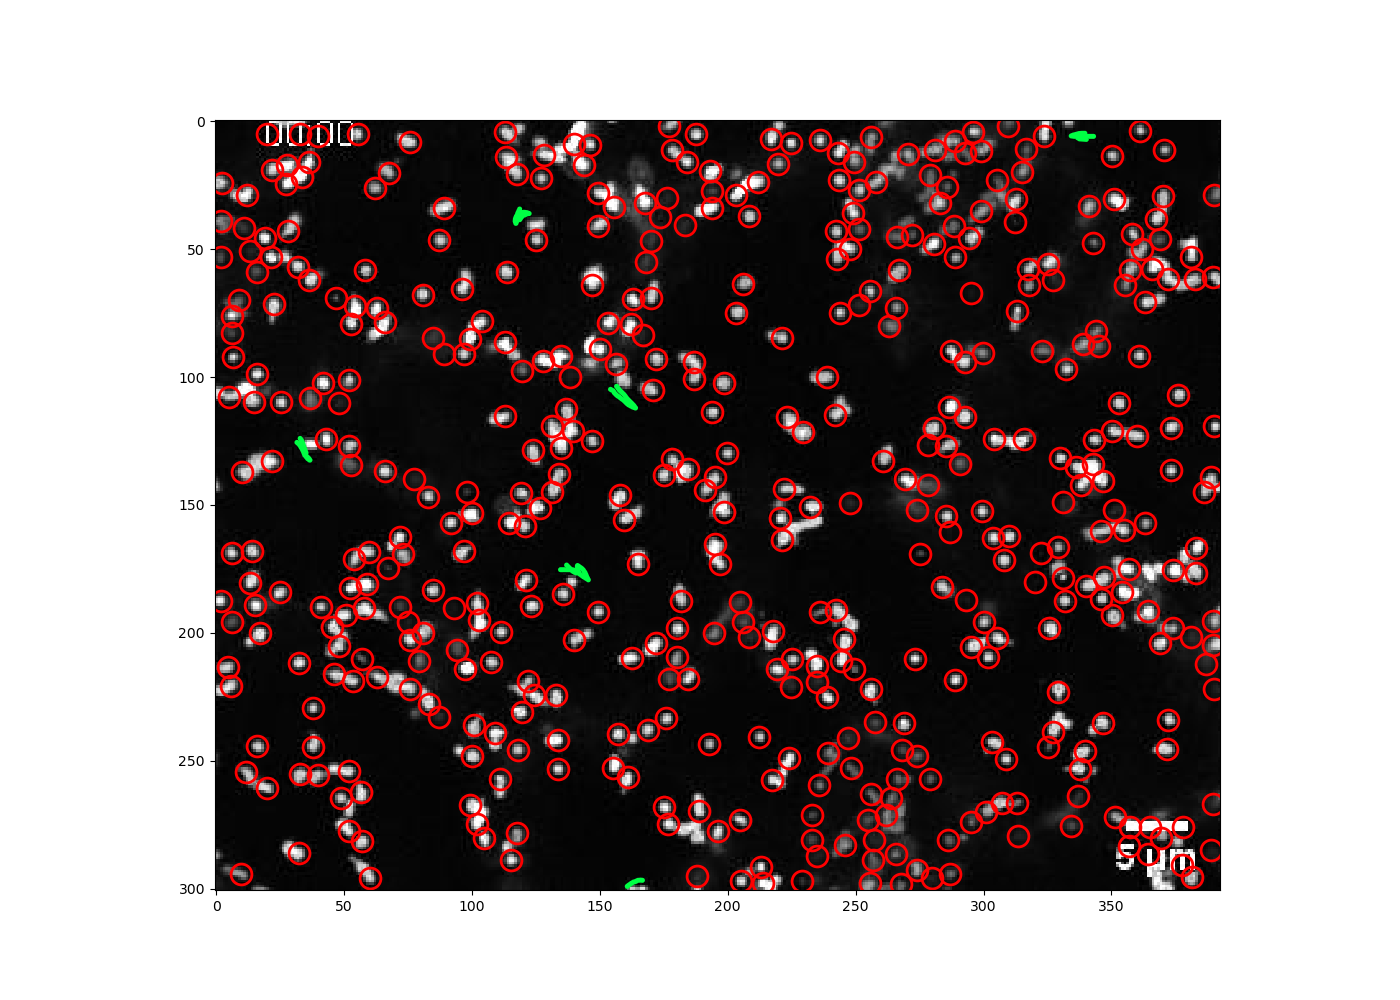
\includegraphics[scale=0.3]{Grafiken/trackpyBilder/locate(frames[0], 5).png}
 	 	\captionof{figure}{locate()-Funktion auf 0. Frame mit diameter=5}
 		 \label{fig:kap3_d=5}
    \end{minipage}
\end{figure}

In Anbetracht des Ziels, einen Durchmesser zu finden, der die Erkennung möglichst vieler Partikel ermöglicht und gleichzeitig möglichst wenig unerwünschte Partikel enthält, ist es besser, mit dem Durchmesser 5 fortzufahren. Denn aus den zuvor verwendeten Durchmessern geht hervor, dass bei diesem Bild die Anzahl der nicht-lokalisierten Teilchen umso größer ist, je höher der Durchmesser ist. 
Dies ist nicht als Allgemeingültigkeit zu verstehen, da verschiedene Videos unterschiedliche Arten von Partikeln mit variierenden Größen und Dicken aufweisen. Es wäre ratsam, die Parameter bei jedem neuen Video zu testen.
Tatsächlich lassen sich insgesamt 475 Partikeln finden, von denen ca. 121 unerwünscht waren und kaum fehlten. Dies entspricht einer ungefähren Rate von 25.47\%.

\begin{figure}[H]
    \centering
    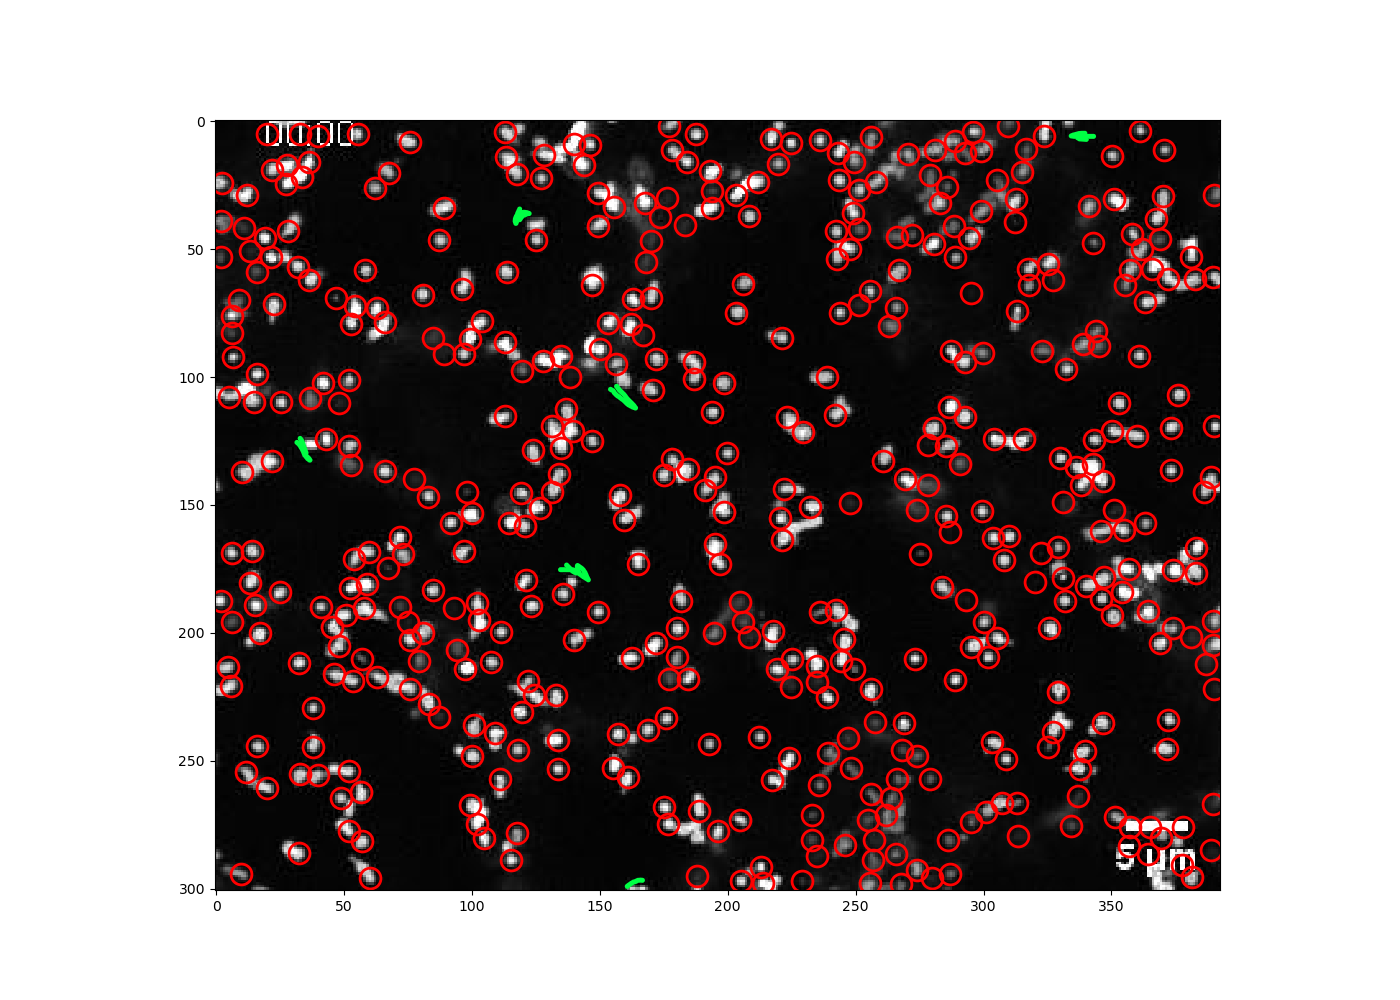
\includegraphics[scale=0.35]{Grafiken/trackpyBilder/locate(frames[0], 5).png}
    \caption{locate()-Funktion auf 0. Frame mit diameter=5}
    \label{fig:kap3_d=5}
\end{figure} 
%    			 In diesem Sinne sieht das Ergebnis der Lokalisierung ohne weitere Parameter wie folgt aus:
%\begin{figure}[H]
%    \centering
%    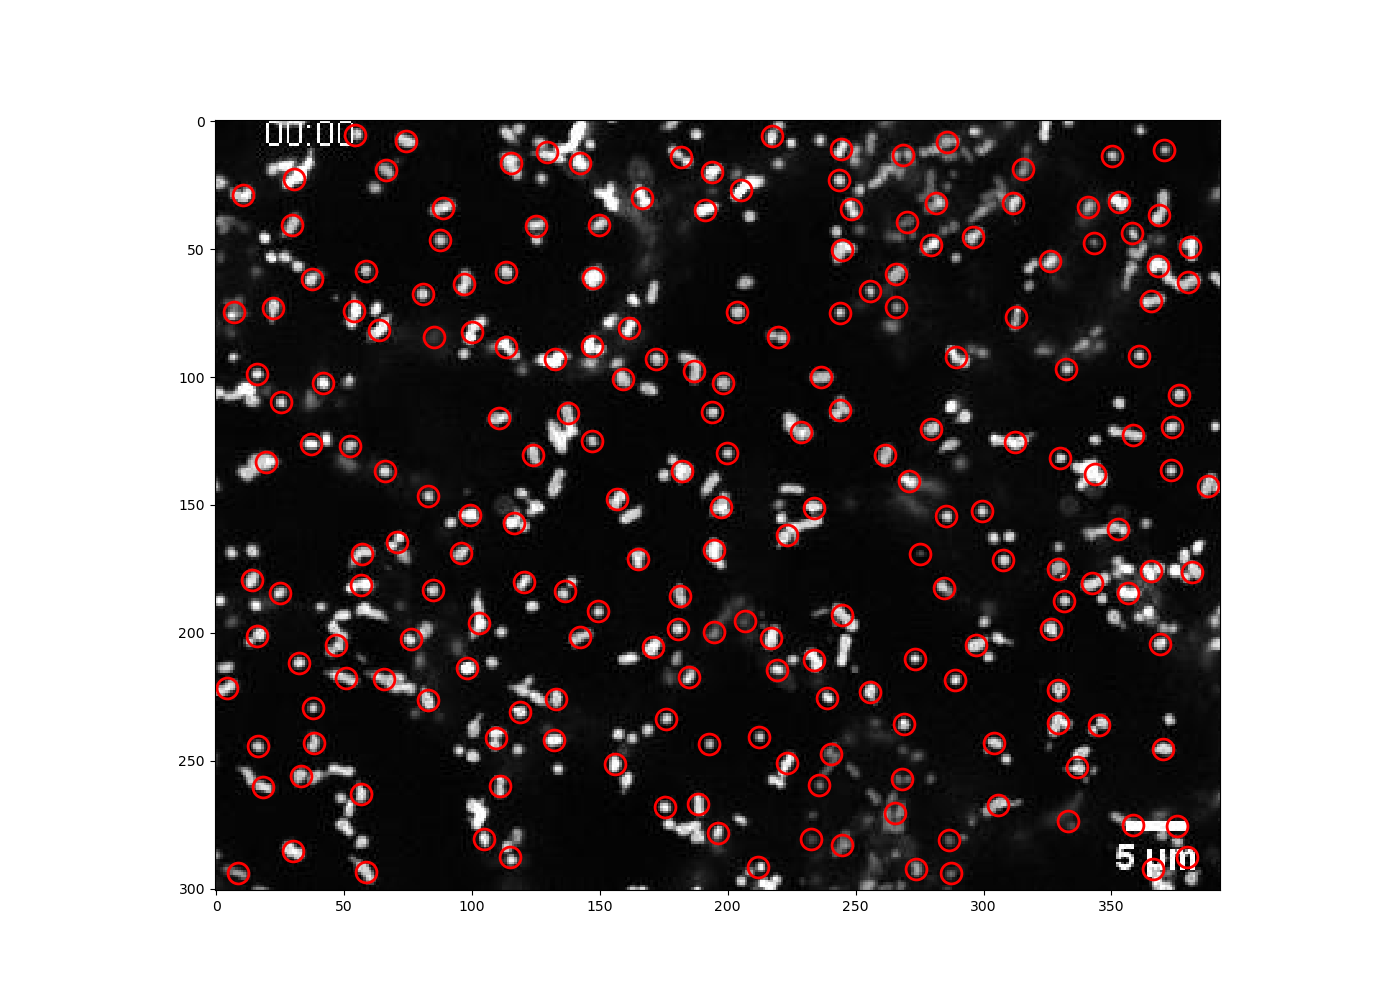
\includegraphics[scale=0.35]{Grafiken/trackpyBilder/locate_with_required_parameter.png}
%    \caption{locate with needed Parameters}
%    \label{fig:bild_label}
%\end{figure}
%    			Wie auf dem \ref{fig:bild_label} zu sehen ist, wurde eine Menge an Partikel 
%    			nicht erkannt, während andere unerwünschten erkannt wurden. 
%    			Insgesamt lassen sich 207 Partikeln finden, von denen 22 unerwünscht waren  und 91 fehlten. Dies entspricht einer ungefähren Rate von 10,628\% für die unerwünschten und einer Rate von 43,9617\% für die nicht gefundenen.

    			
    			\item  {\large \textbf{Ermittlung von \textbf{minmass}}} \\
    			\textbf{locate(f, d, minmass)}:\\ \\
%    			Da ca. nur 10\% der letzten Suche unerwünschte Elemente waren, wird den Durchschnitt der \textit{minmass} aller Teilchen berechnet und als \textit{minmass} verwendet. Aus der vorherigen \textsc{Panda.Dataframe} genügt es den Mittelwert aus den Werten der \textit{mass}-Spalte zu berechnen, um auf \textit{minmass} von ca. 2490.21 zu gelangen. Das Resultat wird dann wie folgt aussehen:
Wie bereits erwähnt, spiegelt \textit{minmass} die inhärente und eingebaute minimale Helligkeit jedes lokalisierten Partikels wider. Das Ziel ist es nun, die zuvor ermittelten, zu dunklen Partikel herauszufiltern. Daher ist es notwendig, methodisch mit dem Parameter \textit{minmass} zu spielen, um dieses Ziel zu erreichen. Es gibt natürlich mehrere Möglichkeiten, den optimalen Wert für die gesuchte Parameter zu finden. Allerdings wird hier die folgende Logik verfolgt:\\

Aus dem DataFrame der letzten Suche (locate(frames[0], 5)) wurde ja 475 Partikel gefunden. Davon sind ca. 25.47\%, also 121 unerwünscht. Diese Zahl entspricht so fast allen gefundenen zu dunklen Partikel. In anderen Worten, stellt sie die Elemente dar, deren \textit{minmass} zu niedrig ist.
So könnte der Dataframe verwendet werden und ihn nach der Spalte \textit{mass} absteigend sortieren. 
Dies würde dazu führen, dass unsere dunkelsten Partikel am Ende der Liste (Tabelle) positioniert werden und die hellsten ganz oben. Dazu muss keine Funktion implementiert werden, sondern es genügt, die Funktion \textit{sort\_values()} aus der Panda. Dataframe-Bibliothek aufzurufen. Der Aufruf sowie die Tabelle sähe jeweils dann wie folgt aus:\\ \texttt{dataframe.sort\_values(by=['mass'], ascending=False)}

\begin{figure}[H]
    \centering
    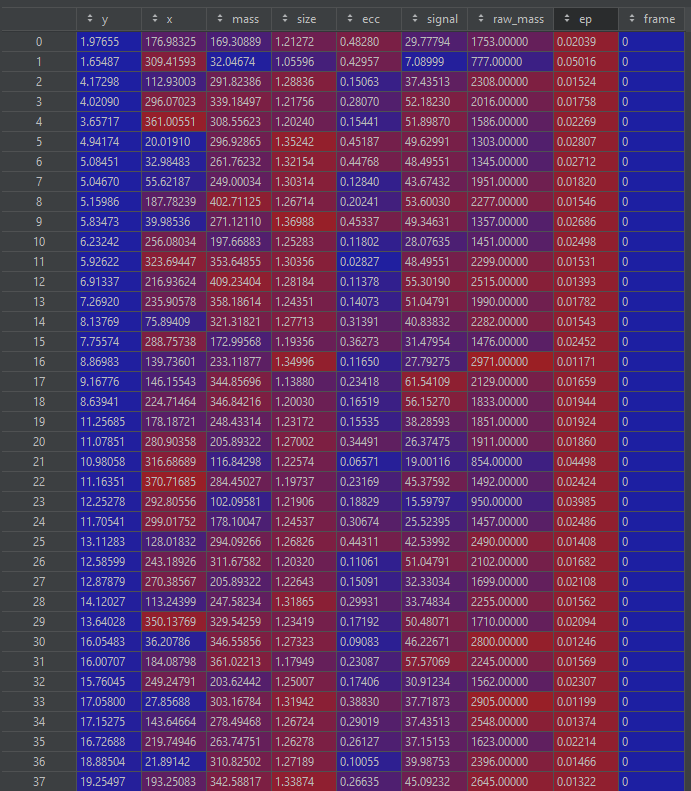
\includegraphics[scale=0.45]{Grafiken/trackpyBilder/df_initial.png}
    \caption{Ein Teil des initialen Dataframes}
    \label{fig:kap3_initDataframe}
\end{figure}

\begin{figure}[H]
    \centering
    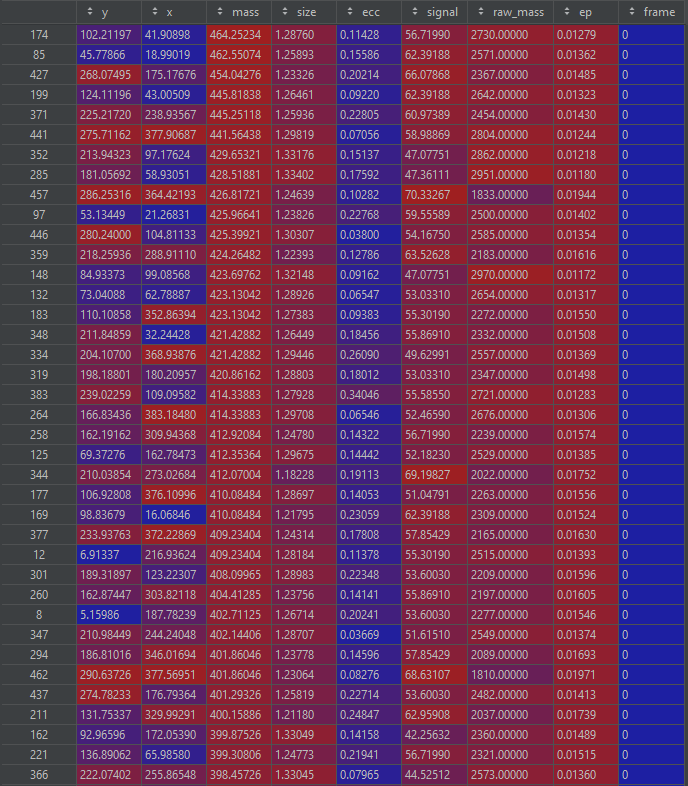
\includegraphics[scale=0.45]{Grafiken/trackpyBilder/df_sorted.png}
    \caption{Ein Teil des sortierten Dataframes}
    \label{fig:kap3_halbsortDataframes}
\end{figure}

Jetzt wird es auf dem sortierten Dataframe eine weitere Funktion aufgerufen, um lediglich nur die 354 (also 475-121)gewünschte Partikel bwz. hellsten zu behalten. Eine solche Funktion \textit{head()} wird auch von Panda-Dataframe bereitgestellt. Aus diesem Ergebnis reicht es aus, die von Python angebotene Funktion \textit{min()} auszuführen, um den kleinsten Wert in der Spalte \textit{mass} zu erhalten. 
Die Aufrufe sähen dann wie folgt aus:\\
\texttt{dataframe.head(354)} \\
\texttt{min(dataframe['mass'])}\\

\textbf{189.72805} ist hier das Ergebnis der vorherigen Vorgänge und damit auch den minimalen Wert von \textit{mass}, den ein Partikel haben muss. Es sei der \textit{minmass} Parameter der Funktion \textit{locate()}.



%Es wurde zwar fast alle \textit{False Positive} beseitigt, aber dafür wurde eine viel zu hohe Anzahl an \textit{True Negative} nicht gefunden. Die Lösung für dieses Problem besteht darin, den Wert von "minmass"  schrittweise zu verringern, bis ein zufriedenstellendes Ergebnis erzielt wird.
\begin{figure}[H]
    \centering
    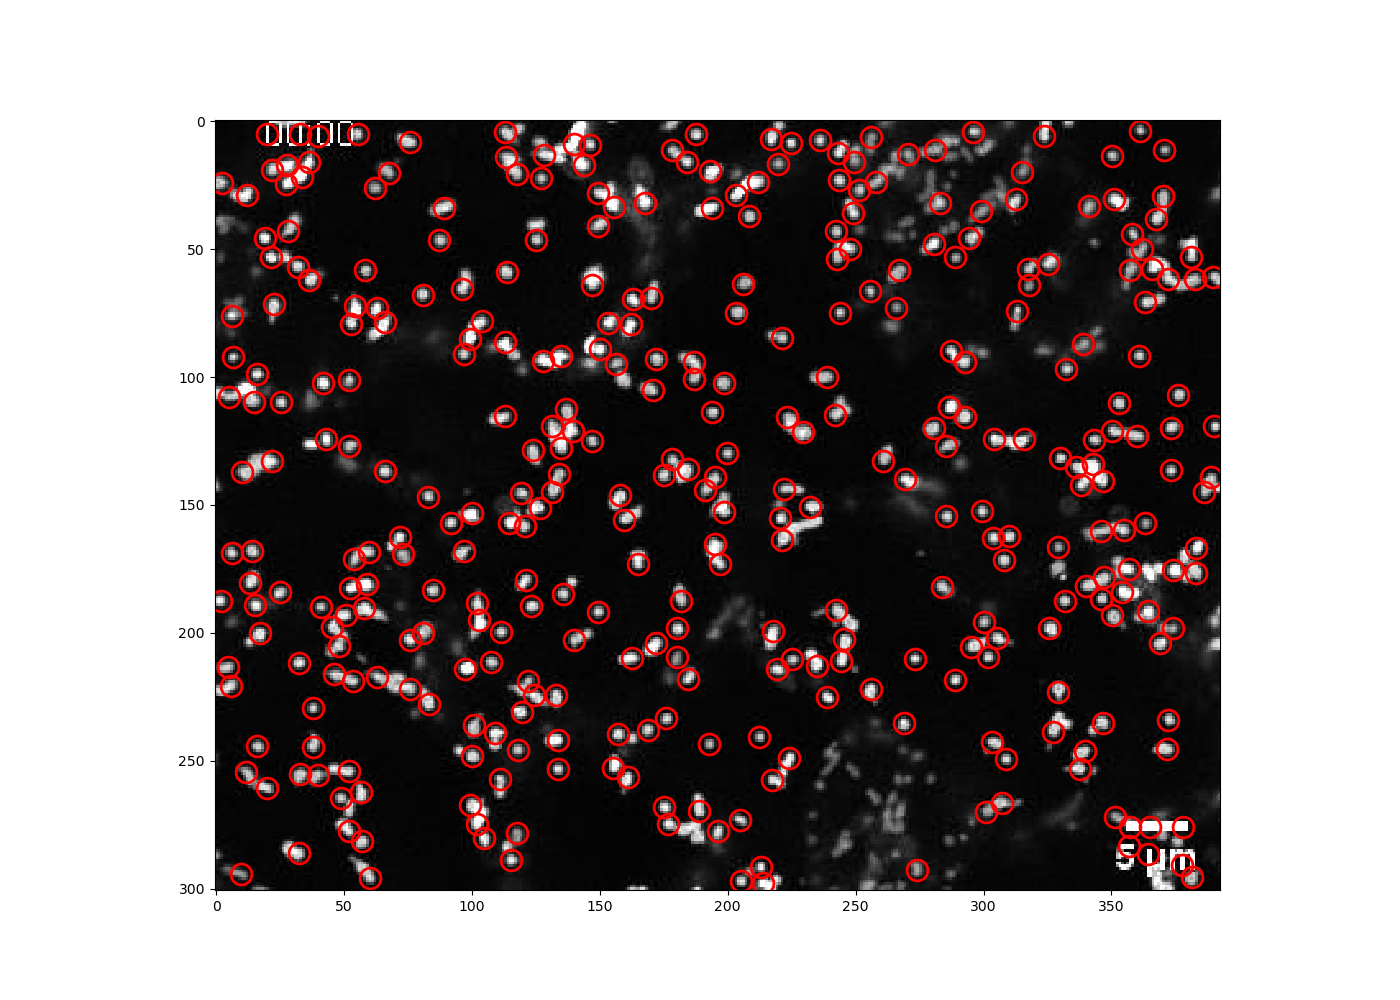
\includegraphics[scale=0.35]{Grafiken/trackpyBilder/locate_with_minmass_01.png}
    \caption{locate()-Funktion auf 0. Frame mit 'mimass=189.72805'}
    \label{fig:kap3_m=189}
\end{figure}

Aus diesem Bild geht hervor, dass fast alle gewünschten Partikel lokalisiert bleiben. Allerdings werden einige von ihnen doppelt gezählt, was Gegenstand der Verwendung anderer Parameter sein wird. Dennoch gibt es noch einige Partikel, die nicht lokalisiert werden sollten. Es handelt sich dabei um etwa 12 Teilchen. Es wäre daher ratsam, die \textit{minmass} schrittweise zu erhöhen, bis ein zufriedenstellendes Ergebnis erzielt wird.\\
Zum Festlegen des Wertes, der in jedem Schritt verwendet werden soll, schauen Sie in der Tabelle (Dataframe), die mit \textit{dataframe.sort\_vaules(by=['mass'], ascending=False}) erstellt wurde, beginnend mit der 121. Zeile von unten nach oben.(121. Zeile entspricht der Anzahl der Teilchen mit geringer Helligkeit)

\begin{figure}[H]
    \centering
    \includegraphics[scale=0.55]{Grafiken/trackpyBilder/df\_steps.png}
    \caption{Sortierte Tabelle}
    \label{fig:kap3_sortDataframes}
\end{figure}

So werden nach und nach die Werte 197,1016 (d. h. 197), 197,6688 (d. h. 198) und so weiter verwendet.\\
Die Verwendung der Funktion \texttt{locate(frames[0], 5, \textbf{minmass=197})} ergibt so gut wie keine Änderung der Lokalisierung. Da insgesamt immer noch 353 Partikel  erkannt wurde. Daher wird sich der nächste Versuch mit dem folgenden Wert beschäftigen. Genauer gesagt "minmass = 198". \\
Auch hier wurden nur zwei Teilchen weniger gefunden. Das sind insgesamt 351 Partikel. Obwohl es fast unmöglich ist, diese beiden Teilchen auf dem Bild zu erkennen. 
Es wäre klug, den nächsten Wert unserer Tabelle zu nehmen, der derzeit bei 203,6244 (also 204) liegt, und erneut zu versuchen, eine Lokalisierung durchzuführen. (Siehe )

\begin{figure}[H]
    \centering
    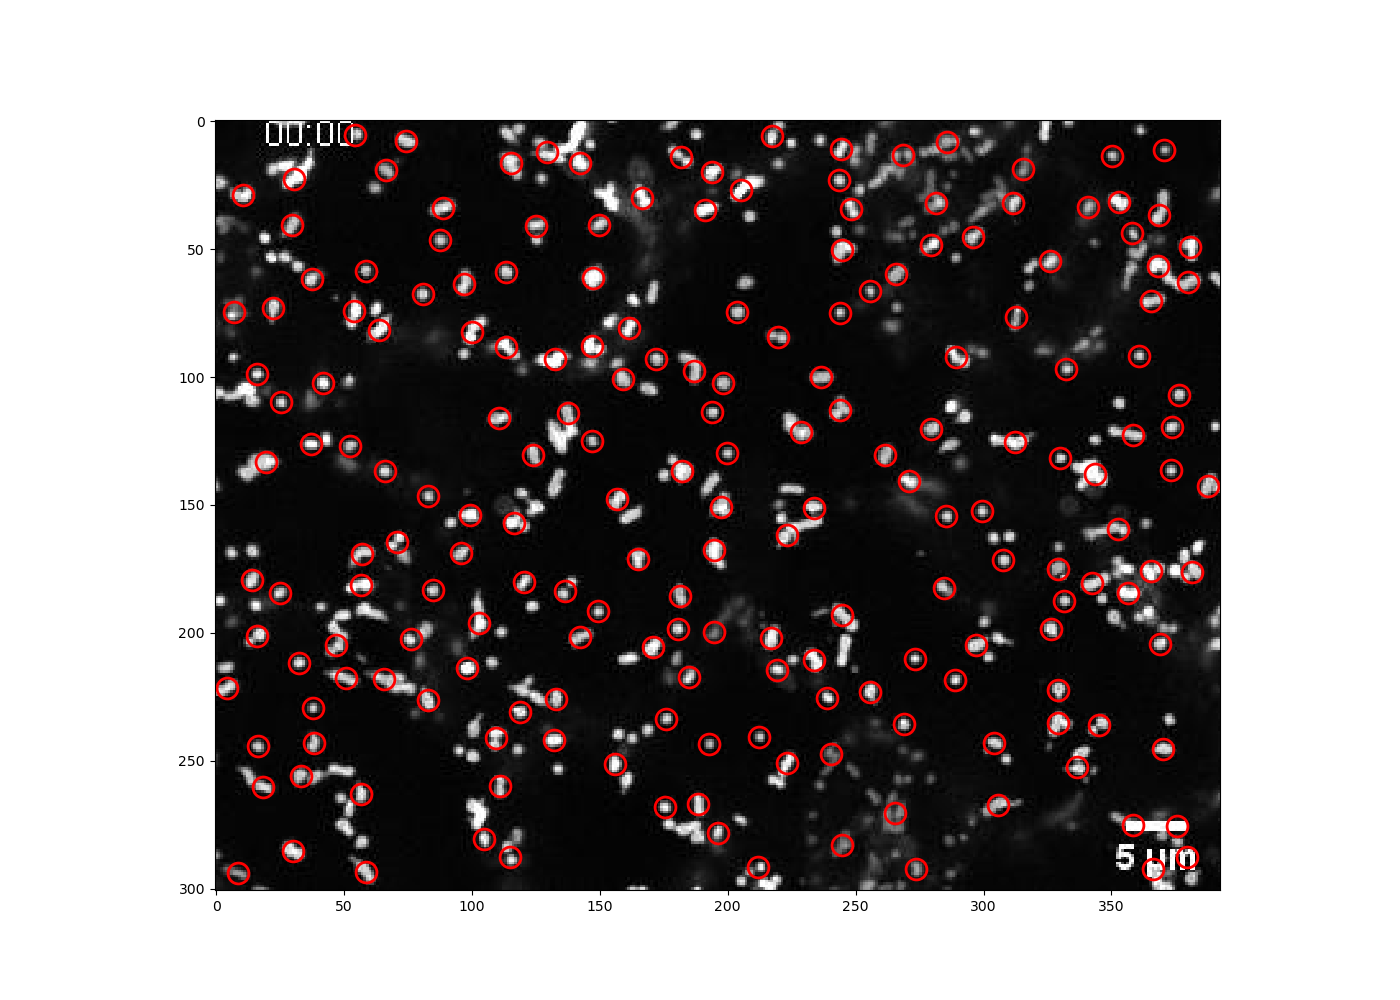
\includegraphics[scale=0.35]{Grafiken/trackpyBilder/locate_with_minmass_02.png}
    \caption{locate()-Funktion auf 0. Frame mit 'mimass=197'}
    \label{fig:kap3_m=197}
\end{figure}


\begin{figure}[H]
    \centering
    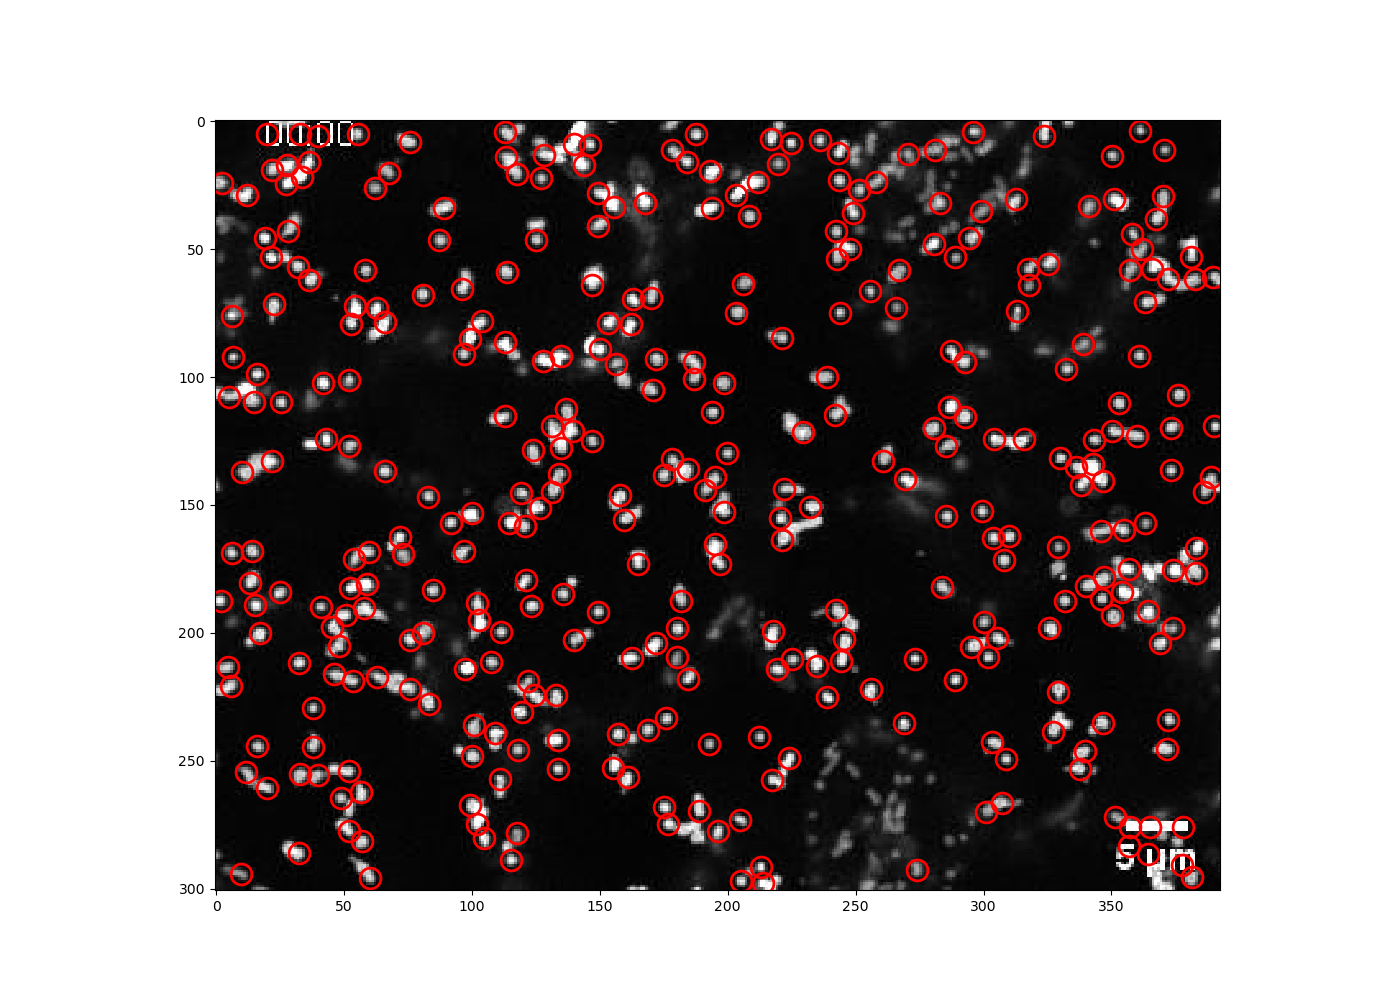
\includegraphics[scale=0.35]{Grafiken/trackpyBilder/locate_with_minmass_04(204).png}
    \caption{locate()-Funktion auf 0. Frame mit 'mimass=204'}
    \label{fig:kap3_m=204}
\end{figure}

Bei der Verfolgung dieser Logik kommt es hier schnell auf einen \textit{minmass} Wert von \textbf{210}.\\
Wo es deutlich zu erkennen ist, dass weitere unerwünschte Partikel nicht mit erkannt wurde. Es wurde insgesamt hier \textbf{345} Partikel gefunden. Jedoch muss es festgestellt werden, dass ab \textbf{211} nach oben, werden zwar weniger unerwünschte Partikel gefangen, aber auch erwünschte. 
Wie es die Veranschaulichung auf Bild (Bild 212)zeigt. 
Deswegen wird es dem weiteren  den Parameter  \textbf{Separation} gewidmet, um weitere unerwünschte zu eliminieren.

\begin{figure}[H]
    \centering
    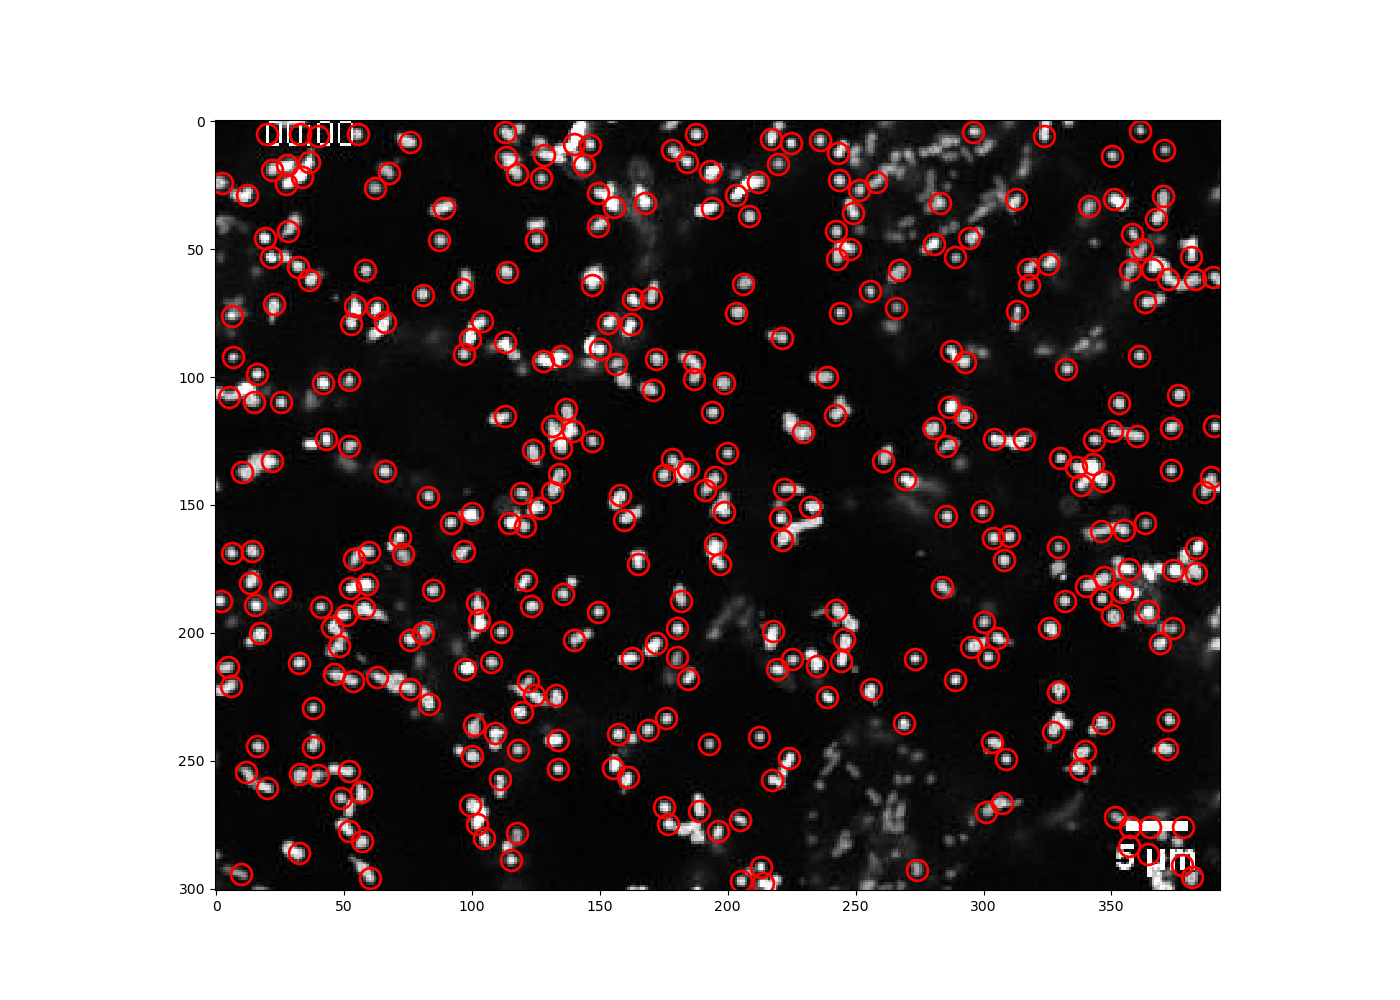
\includegraphics[scale=0.35]{Grafiken/trackpyBilder/locate_with_minmass_07(210).png}
    \caption{locate()-Funktion auf 0. Frame mit 'mimass=210'}
    \label{fig:kap3_m=210}
\end{figure}


\begin{figure}[H]
    \centering
    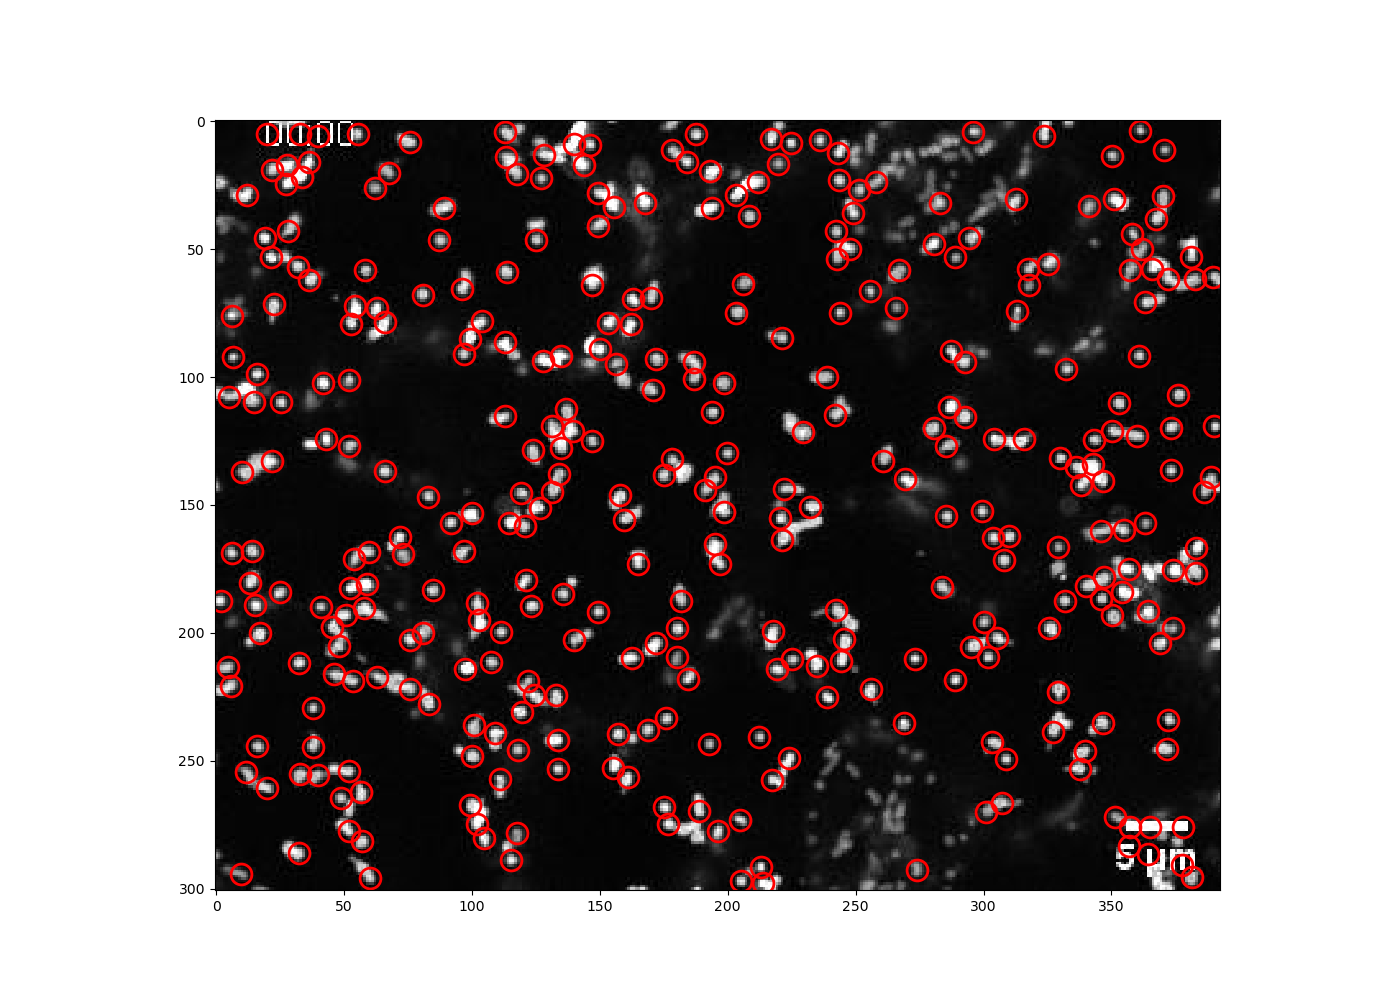
\includegraphics[scale=0.35]{Grafiken/trackpyBilder/locate_with_minmass_08(212).png}
    \caption{locate()-Funktion auf 0. Frame mit 'mimass=212'}
    \label{fig:kap3_m=212}
\end{figure}


		\item {\large \textbf{Ermittlung von \textbf{separation}}} \\
		\textbf{locate(f, d, minmass, separation)} \\ \\
    			Hier wird es einfach Werte bei \texttt{separation} ausprobiert, um auf die bessere Resultate zu kommen. 
    			Es wäre interessant zu erwähnen, dass es sich dabei um den minimalen Abstand zwischen zwei Teilchen handelt. Der Standardwert ist \textit{Durchmesser + 1}. In diesem Fall ist es 6. 
Mit diesem neuen Parameter werden wir versuchen, all jene Partikel zu eliminieren, die doppelt erkannt werden. Ohne die Qualität der bisherigen Erkennung zu beeinträchtigen.  

Denn es scheint offensichtlich, dass, wenn der Wert zu hoch ist, mehrere bisher erkannte Partikel nicht mehr erkannt werden. Weil sie zu nahe beieinander liegen.
Bei \texttt{separation = 6} bleibt die Erkennung unverändert und ergibt auch eine Anzahl von \textbf{345}.

\begin{figure}[H]
    \centering
    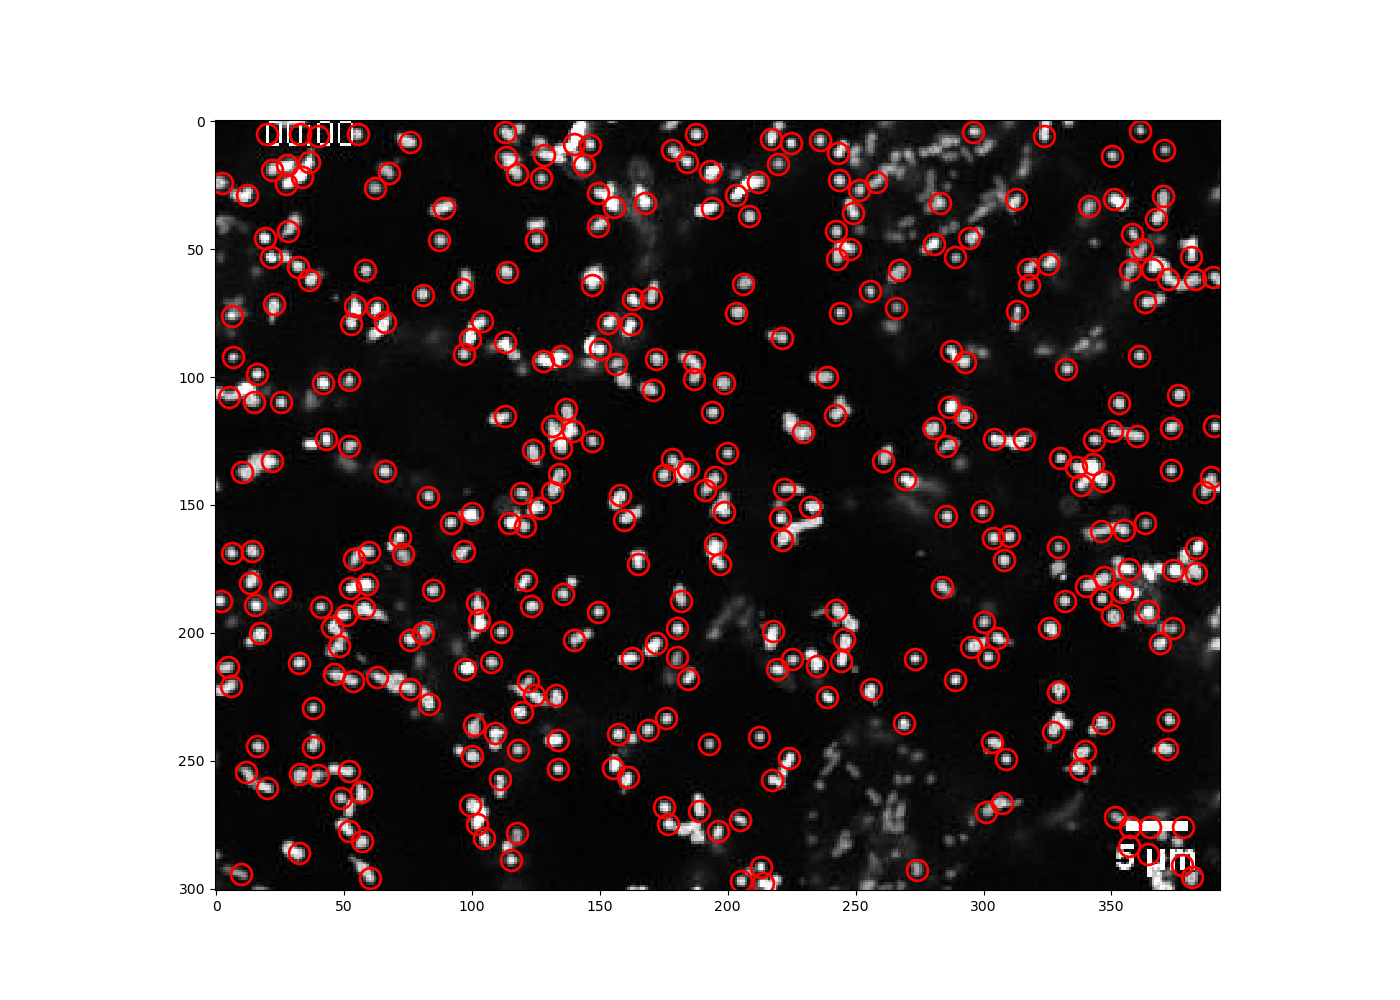
\includegraphics[scale=0.35]{Grafiken/trackpyBilder/locate_with_separation_(6).png}
    \caption{locate()-Funktion auf 0. Frame mit 'separation=6.0'}
    \label{fig:kap3_sep=6}
\end{figure}

Es wird dann als nächstes zuerst \textbf{7} als Parameterwert ausprobieren. Trotz der relativ kleinen Anzahl an insgesamt erkannten Partikel also \textbf{312}. Was auf dem folgenden Bild sichtbar ist, wird es ungefähr \textbf{10} gewünschte Partikel verloren. Diese sind in gelb auf dem Bild markiert. Natürlich hat der Parameterwert nicht nur Verschlechterung gezogen sondern auch positive Effekte. So ist es auch leicht in grün auf dem Bild Ausbesserungen zu sehen. Es handelt sich hier nämlich um \textbf{6} Partikel, die sich mehrfach erkennen lies. 
Allerdings, da die Anzahl an nicht mehr erkannte gewünschte Elemente größer ist als die von nicht gewünschten die eliminiert wurde, wird der Wert des Parameters dann nach unten korrigiert.
\begin{figure}[H]
    \centering
    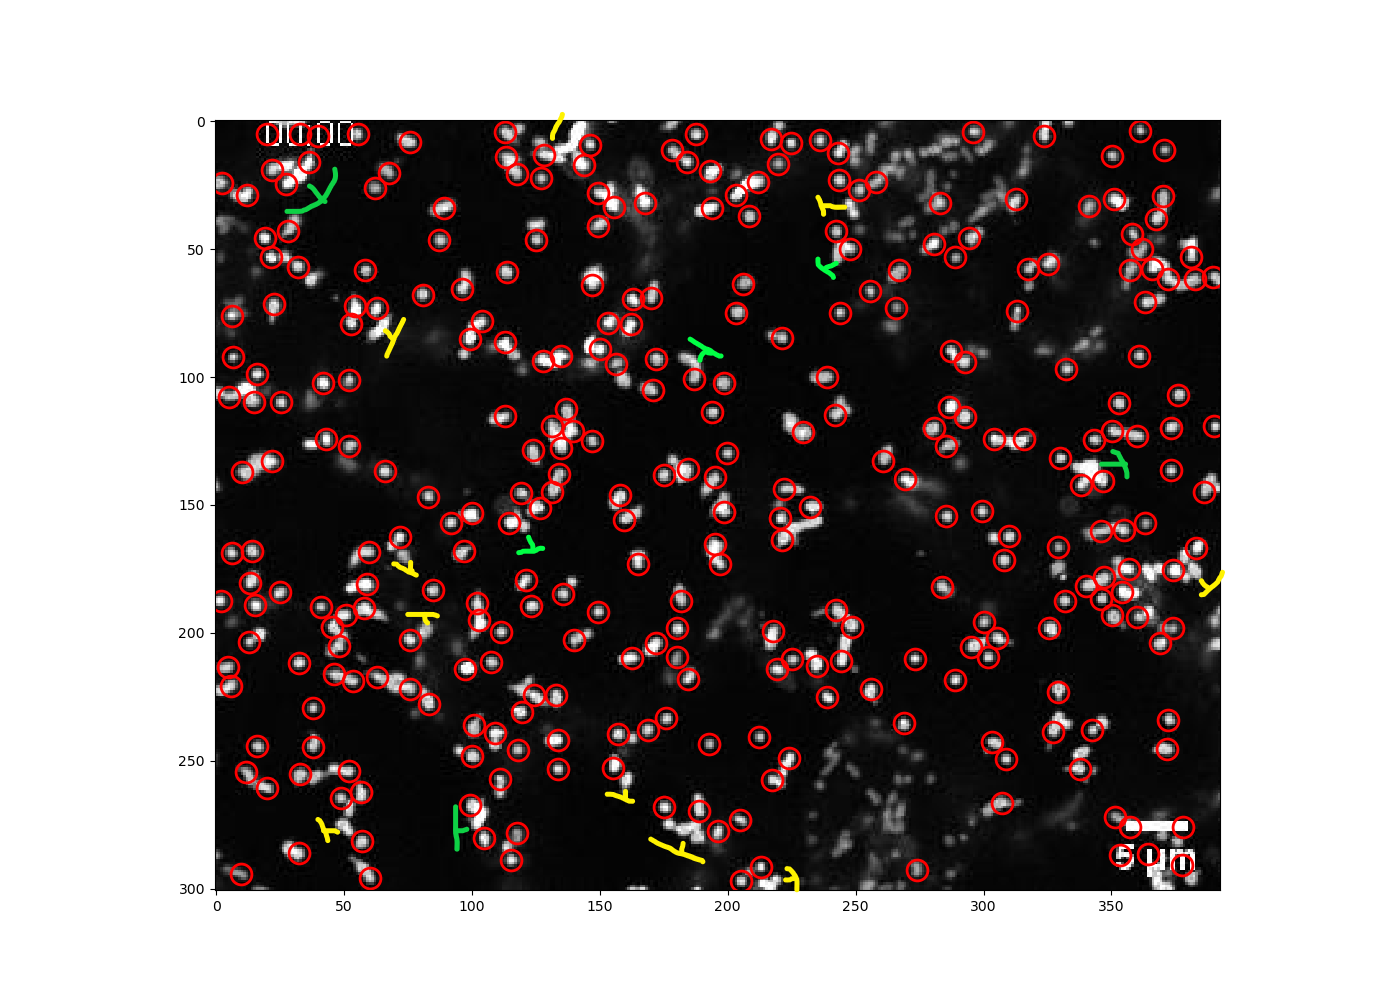
\includegraphics[scale=0.35]{Grafiken/trackpyBilder/locate_with_separation_(7).png}
    \caption{locate()-Funktion auf 0. Frame mit 'separation=7.0'}
    \label{fig:kap3_sep=7}
\end{figure}

Mit den aufeinanderfolgenden Werten \textbf{6.8, 6.7, 6.5 und 6.4} kommt es neben einigen Verbesserungen immer zu mehreren Verschlechterungen, die später mit anderen Parametern nur schwer zu korrigieren sind. 
Genau aus diesem Grund wird hier als  \textbf{separation} der Wert \textbf{6.3} betrachtet.
Wobei fast lediglich nur Verbesserungen zu notieren sind. 
\begin{figure}[H]
    \centering
    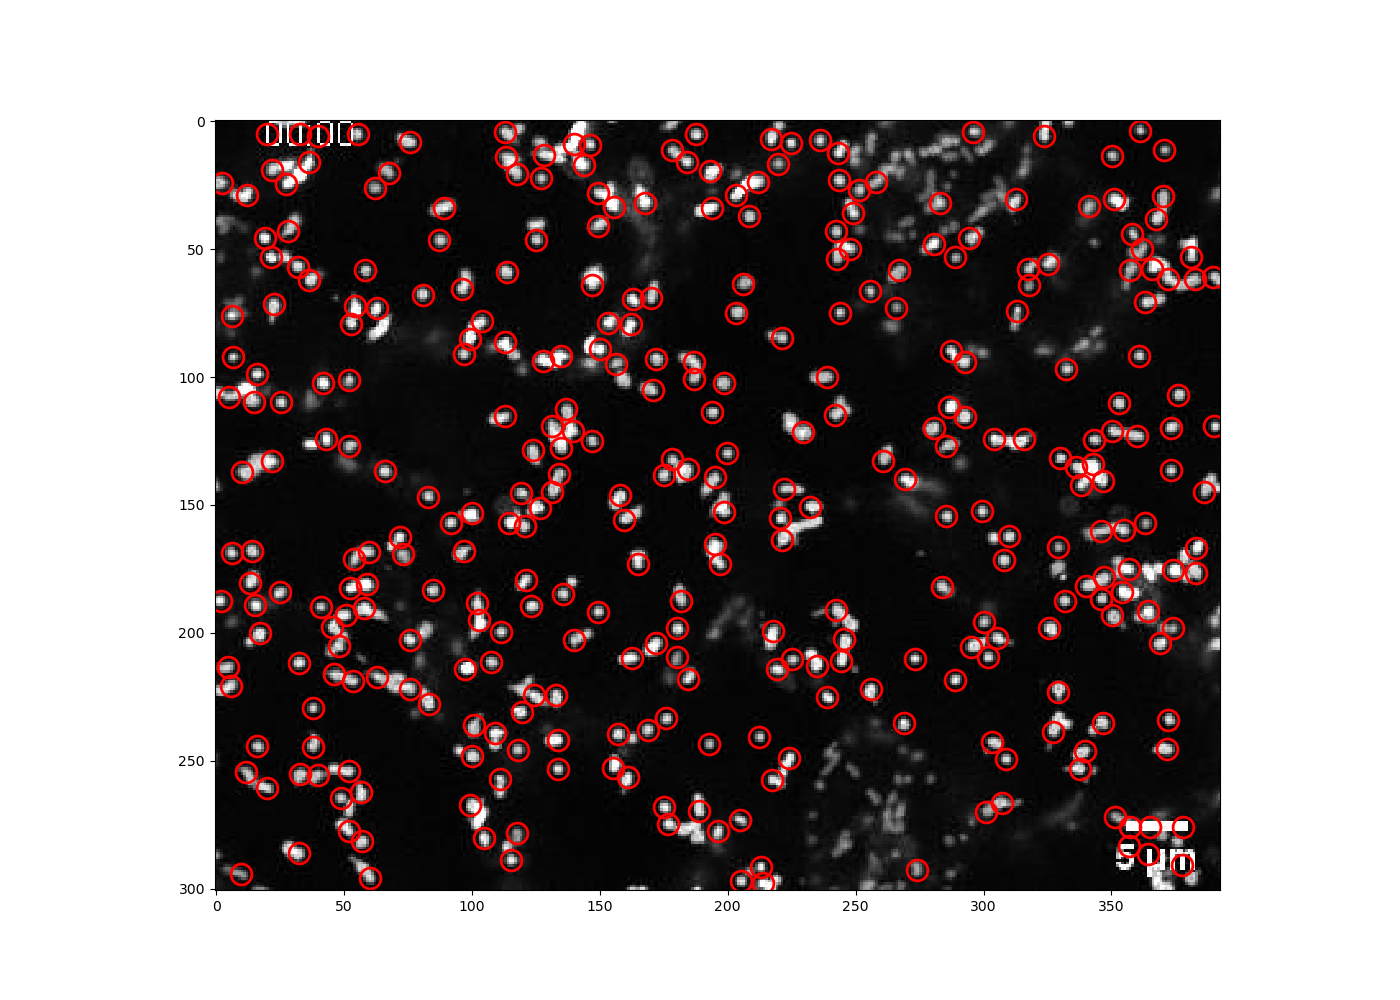
\includegraphics[scale=0.35]{Grafiken/trackpyBilder/locate_with_separation_(6,3).png}
    \caption{locate()-Funktion auf 0. Frame mit 'separation=6.3'}
    \label{fig:kap3_sep=6.3}
\end{figure}


%\item locate(frames[0], 11, minmass=1000.0, separation=2, noise\_size=1.5, topn=250):    \\ \\ 
%		Nachdem alle vorherige Parameter eingesetzt worden sind, wenn der Dataframe immer noch sanierungsbedürftig ist, wird auch \textit{topn} zum Einsatz gebracht. Dazu wird die Anzahl an bestehende unerwünschte Elemente geschätzt und von der gesamten Anzahl an gefundenen Elemente abgezogen. Somit wird \textit{topn} in dem Fall hier auf \textit{250} geschätzt. (siehe Bild)
%\begin{figure}[H]
%    \centering
%    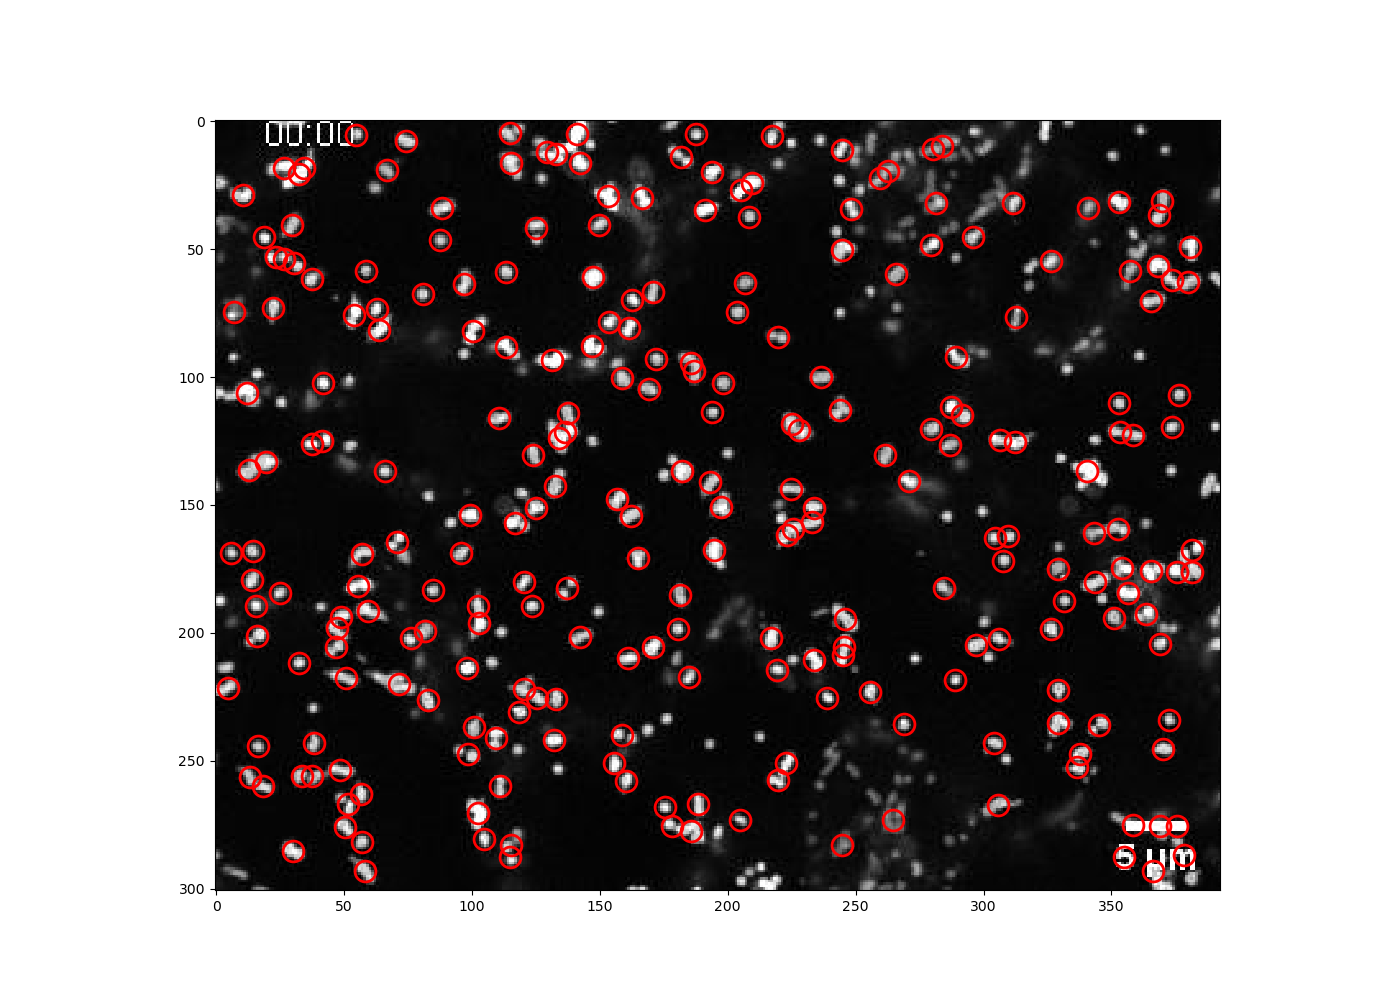
\includegraphics[scale=0.35]{Grafiken/trackpyBilder/locate_with_topn.png}
%    \caption{locate with 'topn=250'}
%    %\label{fig:bild_label}
%\end{figure}
\end{enumerate}


Es scheint hier wichtig zu erwähnen, dass es kein Parameter gibt, dessen Wert adäquat für alle Arten von Bildern oder Partikeln. So sollte es immer Parametrisierung als erster Schritt durchgeführt werden.
Allerdings scheint im konkreten Fall dieses Bildes (nulltes Frames) die Parameterwerte, die am besten geeignet erscheinen, wie folgt: \\
\begin{center}
{\large \textit{locate(frames[0], 5, minmass=210, separation=6.3})}
\end{center}

Diese Werte können jedoch nicht unverändert bleiben, da jedes neue Bild seine eigenen Eigenschaften hat und die Verwendung von Werten, die im Bild \textit{Frame} hervorragende Ergebnisse erzielen, im Bild \textit{Frame+1} zu chaotischen Ergebnissen führen kann.

\begin{figure}[H]
    \centering
    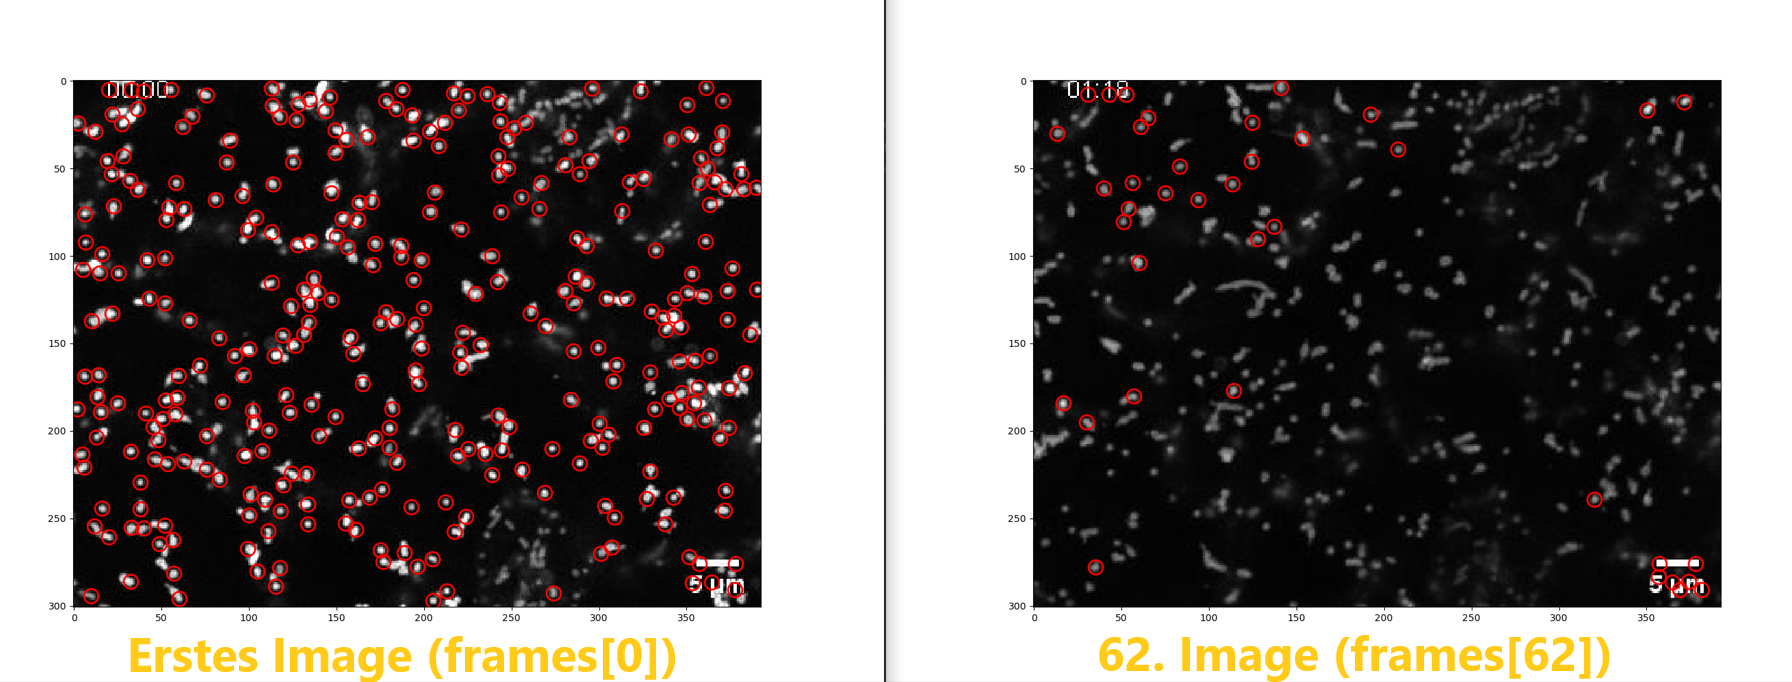
\includegraphics[scale=0.37]{Grafiken/trackpyBilder/comparison_0_Vs_62.png}
    \caption{Vergleich von Bild 1 und Bild 62 mit denselben Parameterwerten.}
    \label{fig:kap3_comp_Bild_1vs_62}
\end{figure}

Tatsächlich wurden auf dem rechten Bild ungefähr 38 Partikel erkannt, während es auf dem linken Bild 335 Partikel waren. Das macht einen Unterschied von 297 Partikeln, obwohl die gleichen Parameter und Werte verwendet wurden.

Die Sicherstellung, dass diese Art von Partikeln, die zwischen den Bildern gefunden werden, nicht mehr reproduziert werden, wird Gegenstand unserer Beschäftigung im nächsten Gliederungspunkt sein.

\section{Automatische Parameter-Optimierung}
Zur Lösung des oben genannten Problems haben wir im Rahmen dieser Arbeit eine Methode namens \textbf{get\_particles\_per\_image\_as\_array} implementiert, die auf alle Bilder des Videos angewendet wird (ein Bild nach dem anderen) und die nach der Bestimmung eines Intervalls sicherstellt, dass die Anzahl der detektierten Partikel in diesem Intervall verbleibt.\\

Das folgende Struktogramm zeigt, wie die Methode sicherstellt, dass die Anzahl der gefundenen Partikel immer innerhalb des zuvor definierten Intervalls bleibt.

An dieser Stelle sei erwähnt, dass das Ergebnis und die Parameter, die zu diesem Ergebnis geführt haben, in einer Variablen mit dem Namen \textbf{particle\_per\_frame} gespeichert werden.  Diese Variable wird auch der Rückgabewert der Funktion sein. 

Außerdem ist der einzige Parameter, der bei der automatischen Optimierung des Ergebnisses berücksichtigt und geändert wird, der "minmass"\-Parameter. Dieser wird verwendet, weil wir im Laufe unserer Versuche festgestellt haben, dass ein Großteil der Ergebnisse nur mit diesem Wert erzielt werden kann.

%Es ist jedoch möglich, verschiedene Werte für bestimmte Parameter zu testen, und zwar für ein bestimmtes Bild mit Hilfe einer anderen Funktion \textbf{update\_frame}.

\begin{figure}[H]
  \centering
  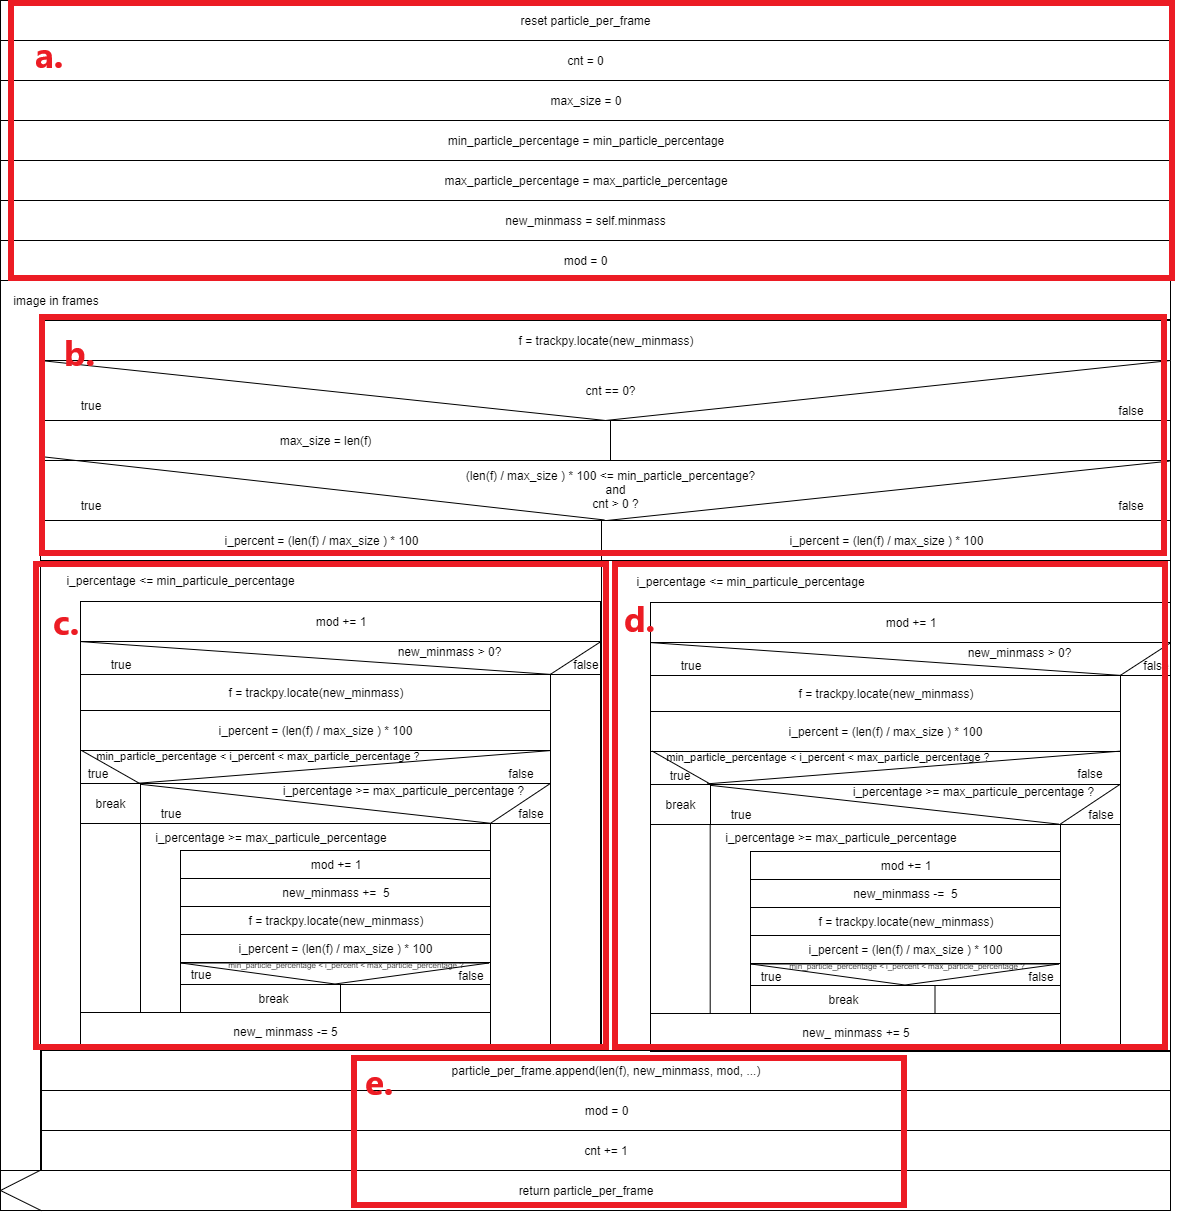
\includegraphics[width=1\textwidth]{Grafiken/pts/structogram.png}
  %\includesvg{Grafiken/pts/structogram.svg}
  \caption{Struktogramm der Methode.: get\_particles\_per\_image\_as\_array()}
  \label{fig:kap3_strukto_part_per_array}
\end{figure}

Das Intervall sollte in Prozent angegeben werden, wobei der Standardwert \textit{80\%} für den unteren Grenzwert und \textit{110\%} für den oberen Grenzwert ist. Die 100\% werden durch die Anzahl der im allerersten Bild erkannten Partikel bestimmt. 
Es wird natürlich davon ausgegangen, dass ein erster Schritt, der manuelle und systematische Suche nach geeigneten Parametern für dieses erste Bild, bereits durchgeführt wurde (\textit{siehe Abschnitt} \ref{kap3_OP}).\\

Nach der Ausführung der Methode mit den Standardprozentwerten für die untere und obere Grenze des Intervalls erhalten wir schließlich das folgende Ergebnis. Dieses Ergebnis wird mit demselben Bild verdeutlicht, bei dem keine automatische Optimierung der Paremeters durchgeführt wurde.

\begin{figure}[H]
    \centering
    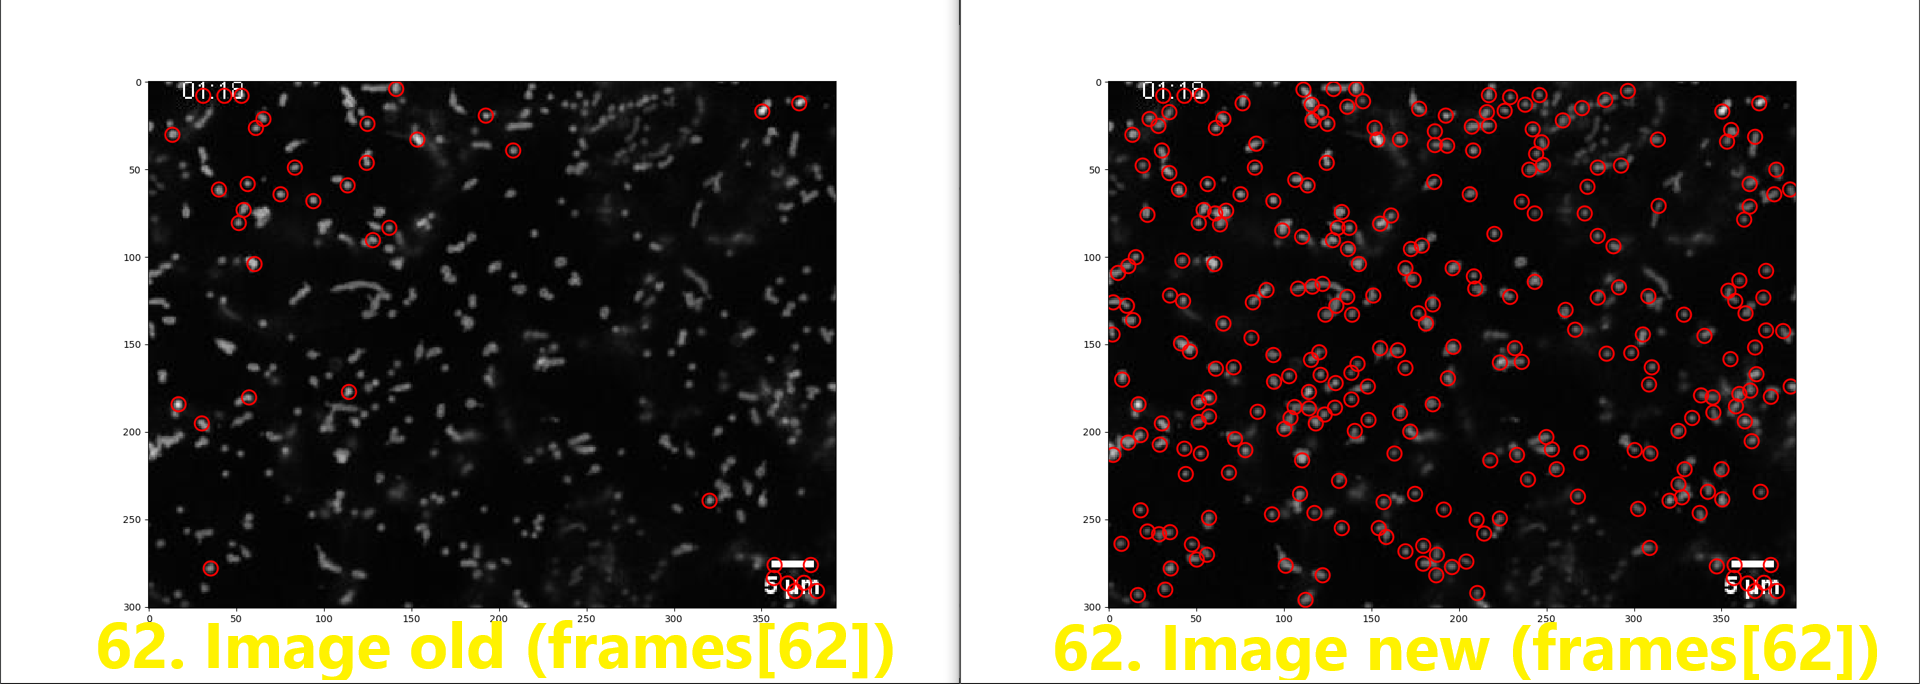
\includegraphics[scale=0.35]{Grafiken/trackpyBilder/comparison_62alt_Vs_62new.png}
    \caption{Vergleich von Bild 62 ohne und mit automatischer Optimierung der Parameter.}
    \label{fig:kap3_vergleich_Bild_62_mit_ohne}
\end{figure}
Es ist jedoch möglich, verschiedene Werte für bestimmte Parameter zu testen, und zwar für ein bestimmtes Bild mit Hilfe einer anderen Funktion \textbf{update\_frame}.

\section{Bearbeitung eines einzelnen Bildes \label{kap3_bearb_einz_bild}}
Die automatische Optimierung hilft zwar dabei, eine gewisse Anzahl von Partikeln in den Ergebnissen zu behalten, aber es kann vorkommen, dass man bei einem bestimmten Bild andere Werte für die Parameter anwenden möchte, ohne die Gesamtheit der enthaltenen Bilder zu verändern. 
Wir haben daher eine Methode namens \textit{\textbf{update\_frame}} entwickelt, mit der wir die gewünschten Änderungen an einem einzelnen Bild vornehmen können.
Sie kann insgesamt 7 Parameter aufnehmen, von denen 2 erforderlich und die anderen 5 optional sind. Die obligatorischen Parameter sind: \textit{frames} und \textit{f\_no}(Die Nummer des zu bearbeitenden Bildes)
Die optionalen sind \textit{minmass}, \textit{separation}, \textit{maxsize}, \textit{topn} und \textit{engine}.

\begin{figure}[H]
  \centering
  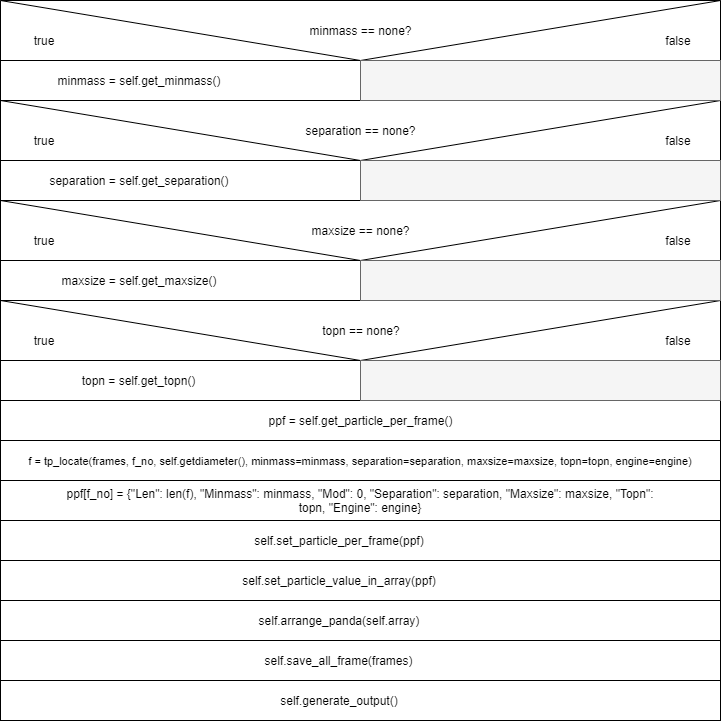
\includegraphics[width=1\textwidth]{Grafiken/pts/update_frame.png}
  %\includesvg{Grafiken/pts/structogram.svg}
  \caption{Struktogramm der Methode: update\_frame()}
  \label{fig:kap3_strukto_update_frame}
\end{figure}

Der obige Struktogramm zeigt, welche Schritte in welcher Reihenfolge ausgeführt werden müssen, um eine Änderung an einem einzelnen Frame vorzunehmen.

So führt die Ausführung des folgenden Codes:\\
\textbf{update\_frame(frames, 66, minmass=170, maxsize=100, topn=150)}\\
Dies bewirkt, dass zuerst die minimale eingebaute Helligkeit auf 170 gesetzt wird, dann der maximale Radius der Helligkeit auf 100 gesetzt wird (so dass keiner der gefundenen Partikel über diesem Wert liegt) und schließlich nur die 150 hellsten Partikel angezeigt werden, die die vorgenannten Bedingungen erfüllen und dies ausschließlich in Frame 66 unseres Videos.


%\subsection{Herausforderungen \& Probleme}

%\subsection{Lösungsansatz \& Umsetzung}

%Glossareintrag \gls{vr}



%\addcontentsline{toc}{chapter}{App}
\chapter{Auswertung}

%\addcontentsline{toc}{section}{App}
\section{App}



%\addcontentsline{toc}{section}{Experimente \& Umsetzung}
%\section{Experimente \& Umsetzung}


%\section{Herausforderungen \& Probleme}
%\addcontentsline{toc}{chapter}{Fazit}
\chapter{Fazit}
Das Ziel unserer Arbeit war es, ein Werkzeug (Software) zu entwickeln, mit dem man in einem bestimmten Video Bild für Bild die vorhandenen Partikel erkennen kann. Anschließend sollte die Anzahl der gefundenen Partikel automatisch konstant gehalten werden (z.B. um zu verhindern, dass durch Lichtveränderungen im Video zu viele Partikel entdeckt werden).\\ Danach sollte eine Benutzeroberfläche entwickelt werden, die es ermöglicht, die Ergebnisse aus den vorherigen Punkten optimal zu bewerten und zu beurteilen. Schließlich sollte auch die Möglichkeit bestehen, die Werte der Parameter, die zu den in den ersten Punkten erzielten Ergebnissen geführt haben, anzupassen, ohne die bereits validierten Ergebnisse zu verändern.\\
Im Kapitel \ref{kap1} haben wir zunächst eine vergleichende Studie verschiedener Werkzeuge durchgeführt, die die Möglichkeit bieten, das erste Ziel (Partikeldetektion) zu erreichen. Dies war \textbf{trackpy}.  Im Kapitel \ref{kap2} stellten wir trackpy vor und berichteten über unsere Erfahrungen als Nutzer.
Erst in Kapitel \ref{kap3} machten wir praktische Fortschritte, indem wir die zu verwendenden Parameter (siehe \ref{kap3_param_loacate}) vorstellten und einen systematischen Weg aufzeigten, wie man angemessene Werte für das erste Bild(Frame) finden kann (siehe \ref{kap3_OP}).\\
 Ebenfalls in diesem Kapitel, im Teil \ref{kap3_OP}, wird erklärt, wie die Lösung, die wir gefunden haben, um die Anzahl der Partikel in einem Intervall zu halten, funktioniert. Der Abschnitt \ref{kap3_bearb_einz_bild} seinerseits behandelt die Frage der Änderung von Parameterwerten und deren Anwendung in unserem Kontext.\\
Schließlich zeigen wir im Kapitel \ref{kap6} den Installationsprozess sowohl des Frontends als auch des Backends unseres Tools (Software). Wir haben auch die von uns entworfene Benutzeroberfläche vorgestellt, die unserer Meinung nach optimal für die Visualisierung und Bewertung der Parameterwerte ist, die zur Erzielung von Ergebnissen verwendet werden.


%\addcontentsline{toc}{section}{Fazit}
%\section{Fazit}

%\addcontentsline{toc}{section}{Eigene Meinung/Reflektion}
%\section{Eigene Meinung/Reflektion}
%\addcontentsline{toc}{chapter}{Ausblick}
\chapter{Ausblick}

Ausblick
%\input{Kapitel/Kapitel-7/kapitel-7}

\phantomsection

%%%%%%%%%%%%%%Anhang%%%%%%%%%%%%%%

%Abbildungsverzeichnis
\addcontentsline{toc}{chapter}{Abbildungsverzeichnis}
\listoffigures

\phantomsection

%Tabellenverzeichnis
\addcontentsline{toc}{chapter}{Tabellenverzeichnis}
\listoftables

\phantomsection

%Algorithmen
\addcontentsline{toc}{chapter}{Algorithmen}
\chapter*{Algorithmen}

Algorithmen

\phantomsection

%Glossar
\printglossary

\phantomsection

%Quellenverzeichnis
\addcontentsline{toc}{chapter}{Literaturverzeichnis}
\bibliography{quellenverzeichnis}

\phantomsection

%Anhang
\addcontentsline{toc}{chapter}{Anhang}
\chapter*{Anhang}

Anhang

%\phantomsection

\end{document}
